% IACR Transactions CLASS DOCUMENTATION
% Written by Gaetan Leurent gaetan.leurent@inria.fr (2016-2018)
%
% To the extent possible under law, the author(s) have dedicated all
% copyright and related and neighboring rights to this software to the
% public domain worldwide. This software is distributed without any
% warranty.
%
% You should have received a copy of the CC0 Public Domain Dedication
% along with this software. If not, see
% <http://creativecommons.org/publicdomain/zero/1.0/>.

\documentclass[preprint]{iacrtrans} 
\usepackage[utf8]{inputenc}

\setcounter{tocdepth}{4}

%% VERSION 
\newcommand{\version}{v.1.0}


%% TITLE
\title{
	
\includegraphics[width=\columnwidth]{logo_zkEVM.png} 	\\ \vspace{0.3cm}
	Technical Document 										\\ \vspace{0.3cm}	
	eSTARK: Extending the STARK Protocol with Arguments		\\ \vspace{0.3cm}
	\version
}

\institute{}


\usepackage{caption}
\usepackage{subcaption}

% This package controls how hyperlinks are displayed
% https://es.overleaf.com/learn/latex/Hyperlinks
\usepackage{hyperref}
\hypersetup{colorlinks=true,linkcolor={red!80!black},urlcolor={blue!80!black}}

%Multiple columns
\usepackage{multicol}

% Used for super caligraphic font \mathscr{}
\usepackage{mathrsfs} 

%This ensures spaces when using ensuremath and no $$ are used to introduce math
\usepackage{xspace}

%%%%%% BEGIN OF CODE HIGHLIGHTING ENVIRONMENTS %%%%%%

%   sudo apt install texlive-latex-extra 
%   sudo apt install python-pip
%   pip install pygments
%   pip install pygments-lexer-babylon  #contains JSX
%   pip install pygments-lexer-solidity 
%   pip install pygments pygments-lexer-babylon pygments-lexer-solidity

%%%%%%% IF STATEMENTS %%%%%%%%%%%
\newif\ifSOUNDNESS
\newif\ifPOLYGON
\POLYGONtrue

\newif\ifNOPOLYGON
\NOPOLYGONfalse

% *** COLOR COMMANDS ***
\definecolor{dblackcolor}{rgb}{0.0,0.0,0.0}
\definecolor{dbluecolor}{rgb}{0.01,0.02,0.5}
\definecolor{dgreencolor}{rgb}{0.2,0.4,0.0}
\definecolor{dgraycolor}{rgb}{0.30,0.3,0.30}
\newcommand{\dblue}{\color{dbluecolor}\bf}
\newcommand{\dred}{\color{dredcolor}\bf}
\newcommand{\dblack}{\color{dblackcolor}\bf}
\definecolor{light-gray}{gray}{0.96} %the shade of grey that stack exchange uses

%Linter for circom
\usepackage{listings}
\lstdefinelanguage{circom}[]{C}{
	morekeywords = {component, include, input, function, output, parallel, pragma, public, private, signal, template, var}, 
	sensitive=true}
\lstset{
	backgroundcolor = \color{light-gray},
	showtabs = False,
	tabsize = 2,
	showspaces = False,
	showstringspaces = False,
	commentstyle = {\ttfamily\color{dgreencolor}},
	keywordstyle = {\ttfamily\color{dbluecolor}\bfseries},
	stringstyle = {\ttfamily\color{dgraycolor}\bfseries},
	language = circom,
	basicstyle = {\fontsize{7pt}{7pt}\ttfamily},
	aboveskip = 1em,
	belowskip = 1em,
	numbers = left,%none,
	numbersep=5pt,    %space line numbers from code
	xleftmargin=2em,
	frame=single,	% adds a frame around the code
	framexleftmargin=1.7em,
	numberstyle=\tiny,%\color{gray}
	emph = {proc,retp,endp,local}, 
	emphstyle = {\color{blue}\textbf},
	literate = 	
		{<==}{{{\color{dbluecolor}<==}}}2 
		{==>}{{{\color{dbluecolor}==>{}}}}2
		{===}{{{\color{dbluecolor}==={}}}}2
		{<--}{{{\color{dbluecolor}<---{}}}}2
		{-->}{{{\color{dbluecolor}--->{}}}}2
		{*}{{{\color{dbluecolor}*{}}}}2
}

%%%%%%% END OF CODE HIGHLIGHTING ENVIRONMENTS %%%%%%%



%%%%%%%%%%%%%%%%%%% BEGIN OF MACROS %%%%%%%%%%%%%%%%%%%

% Cryptocode: https://github.com/arnomi/cryptocode
\usepackage[
lambda,
operators,
landau, %este es el de bigO
probability,
%sets,
logic, %para or,and...	
asymptotics,
keys
]{cryptocode}

% My own procedure blocks to show protocols
\createprocedureblock{mypb}{center, boxed}{}{}{linenumbering}
\createprocedureblock{mypbnonum}{center, boxed}{}{}{}

% Numbering style
\renewcommand{\pclnstyle}[1]{\text{#1}}
\renewcommand{\pclnseparator}{.}

% Hyphen inside mathmode
\mathchardef\mhyphen="2D

% Mathbb
\newcommand{\FF}{\ensuremath{\mathbb{F}}\xspace}
\newcommand{\KK}{\ensuremath{\mathbb{K}}\xspace}
\newcommand{\NN}{\ensuremath{\mathbb{N}}\xspace}
\newcommand{\ZZ}{\ensuremath{\mathbb{Z}}\xspace}

% Mathcal
\newcommand{\A}{\ensuremath{\mathcal{A}}\xspace}
\newcommand{\C}{\ensuremath{\mathcal{C}}\xspace}
\newcommand{\E}{\ensuremath{\mathcal{E}}\xspace}
\newcommand{\F}{\ensuremath{\mathcal{F}}\xspace}
\renewcommand{\H}{\ensuremath{\mathcal{H}}\xspace}
\newcommand{\I}{\ensuremath{\mathcal{I}}\xspace}
\renewcommand{\O}{\ensuremath{\mathcal{O}}\xspace}
\renewcommand{\P}{\ensuremath{\mathcal{P}}\xspace}
\newcommand{\R}{\ensuremath{\mathcal{R}}\xspace}
\renewcommand{\S}{\ensuremath{\mathcal{S}}\xspace}
\newcommand{\T}{\ensuremath{\mathcal{T}}\xspace}
\newcommand{\V}{\ensuremath{\mathcal{V}}\xspace}

% Mathscr
% \newcommand{\PPP}{\ensuremath{\mathscr{P}}\xspace}


% Mathfrak
\newcommand{\afr}{\ensuremath{\mathfrak{a}}\xspace}
\newcommand{\bfr}{\ensuremath{\mathfrak{b}}\xspace}

% Caligraphic Combiantions
\DeclareMathAlphabet{\mathpgoth}{OT1}{pgoth}{m}{n}
\newcommand{\plonk}{\ensuremath{\mathcal{P}\mathfrak{lon}\mathcal{K}}\xspace}
\newcommand{\plookup}{\ensuremath{\mathpgoth{plookup}}\xspace}

% Abbreviations
% \newcommand{\Pp}{\ensuremath{\mathcal{P}_{\textsf{poly}}\xspace}}
\newcommand{\MTR}{\ensuremath{\text{MTR}}\xspace}
\newcommand{\MTP}{\ensuremath{\text{MTP}}\xspace}
\newcommand{\LCC}{\ensuremath{\text{LCC}}\xspace}
\newcommand{\FRI}{\ensuremath{\textsf{F}}\xspace}
\newcommand{\z}{\ensuremath{\overline{z}}\xspace}
\newcommand{\fsel}{\ensuremath{f^{\text{sel}}}\xspace}
\newcommand{\tsel}{\ensuremath{t^{\text{sel}}}\xspace}
\newcommand{\Evals}{\ensuremath{\textsf{Evals}}\xspace}
\newcommand{\pparams}{\ensuremath{\text{pp}}\xspace}
\newcommand{\vparams}{\ensuremath{\text{vp}}\xspace}
\newcommand{\pre}{\ensuremath{\text{pre}}\xspace}
\newcommand{\tr}{\ensuremath{\text{tr}}\xspace}
\newcommand{\otr}{\ensuremath{\overline{\text{P}}}\xspace}
\newcommand{\im}{\ensuremath{\text{im}}\xspace}
\newcommand{\seed}{\ensuremath{\textsf{seed}}\xspace}
\newcommand{\transcript}{\ensuremath{\textsf{transcript}}\xspace}
\newcommand{\AIR}{\ensuremath{\textsf{A}}\xspace}
\newcommand{\eAIR}{\ensuremath{\textsf{eA}}\xspace}
\newcommand{\accept}{\ensuremath{\textsf{accept}}\xspace}
\newcommand{\reject}{\ensuremath{\textsf{reject}}\xspace}
\newcommand{\eFRI}{\ensuremath{\epsilon_{\textsf{FRI}}}\xspace}
\newcommand{\eSTARK}{\ensuremath{\epsilon_{\textsf{STARK}}}\xspace}
\newcommand{\eeSTARK}{\ensuremath{\epsilon_{\textsf{eSTARK}}}\xspace}
\newcommand{\eC}{\ensuremath{\epsilon_{\textsf{C}}}\xspace}
\newcommand{\ePlo}{\ensuremath{\epsilon_{\textsf{Plo}}}\xspace}
\newcommand{\eMulEq}{\ensuremath{\epsilon_{\textsf{MulEq}}}\xspace}
\newcommand{\eCon}{\ensuremath{\epsilon_{\textsf{Con}}}\xspace}
\newcommand{\eArgs}{\ensuremath{\epsilon_{\textsf{Args}}}\xspace}
\newcommand{\RS}{\ensuremath{\textsf{RS}[\FF,H,\rho]}\xspace}
\newcommand{\RSK}{\ensuremath{\textsf{RS}[\KK,H,\rho]}\xspace}
\newcommand{\LH}{\ensuremath{\textsf{LH}}\xspace}
\newcommand{\ID}{\ensuremath{\textsf{ID}}\xspace}

% Polygon Commands
\newcommand{\transcriptAdd}{\ensuremath{\textsf{add}_{\transcript}}\xspace}
\newcommand{\transcriptExtract}[1]{\ensuremath{\mathsf{extract}_{#1}\xspace}}

% Make a nice emptyset
\let\oldemptyset\emptyset
\let\emptyset\varnothing

% Make a nice phi and epsilon
\let\oldphi\phi
\let\phi\varphi
\let\oldepsilon\epsilon
\let\epsilon\varepsilon

% Make a nice q.e.d. symbol
\renewcommand\qedsymbol{\ensuremath{\blacksquare}\xspace}

\theoremstyle{definition}
\newtheorem{protocol}{Protocol}
\newtheorem{bremark}{Remark}

%%%%%%%%%%%%%%%%%%% END OF MACROS %%%%%%%%%%%%%%%%%%%

% \begin{pcvstack}[boxed, center]
% % \pcsetargs{codesize=\scriptsize{}}

% \procedure{}{
%   \textbf{Prover } \P(g_1(x))  \< \< \textbf{verifier } \V(g_1(x)) \\[][\hline]
%   \< \sendmessageright{top={$f_1(s)$, $f_2(s)$}} \< \\[-2mm]
%   \< \sendmessageleft{top={randomness}} \< \\[-2mm]
%   \< \sendmessageright{top={$f_3(s)$}} \< \\[-2mm]
%   \< \< \text{Samples a random } z \in \FF \text{ and computes } z\vec{g}. \\[-2mm]
%   \< \sendmessageleft{top={$z$}} \< \\[-2mm]
%   \text{Computes evaluations:} \< \< \\
%   \t g_1(z), f_1(z), f_2(z), f_3(z) \< \< \\[-2mm]
%   \< \sendmessageright{top={$g_1(z)$, $f_1(z)$, $f_2(z)$, $f_3(z)$}} \< \\[-2mm]
%   \< \sendmessageleft{top={$v$}} \< \\[-2mm]
%   \< \sendmessageright{top={$\pi$}} \< \\[-2mm]
%   \< \< \text{Verifies the opening proof } \pi \text{ and checks that:} \\
%   \< \< \t g_1(z)(f_1(z) + f_2(z)) - f_3(z) = 0
% }
% \end{pcvstack}

\begin{document}

\begin{titlepage}
\centering
\maketitle
\today
\vspace{-5mm}
\end{titlepage}

% use optional argument because the \LaTeX command breaks the PDF keywords
% \keywords[\publname, ToSC, TCHES, LaTeX]{TBD \and TBD}

{\hypersetup{linkcolor=.}\tableofcontents}

\newpage


\section{Background}

%%%%%%%%%%%%%%%%%%%%%%%%%%%%%%%%%%%%%%%%%%%%%%%%%%%%%%%%%%%%%%%%%%%%%%%%%%%%%%%%
\subsection{Terminology and Conventions}

Let $n,n_1,n_2 \in \NN$ such that $n_1 < n_2$. We often denote by $[n]$ to the set $\{1,2,\dots, n\}$ and by $[n_1,n_2]$ to the set $\{n_1, n_1+1, \dots, n_2 - 1, n_2\}$.

We denote by $\FF$ to a finite field of prime order $p$ and by $\FF^*$ to its respective multiplicative group. We also write $\FF[X]$ for the ring of polynomials with coefficients over $\FF$ and write $\FF_{<d}[X]$ to denote the set of polynomials of degree lower than $d$. Given a positive integer $N$, we always assume the existence of a cyclic subgroup $G$ of $\FF^*$ and denote by $g \in \FF$ to its generator.

In PIL we treat polynomials and entire columns of execution traces indistinguishably for the following reason. Given a column $\att$ of length $N$, which can be viewed as the vector $(a_1,\dots,a_N)$ with $a_i \in \FF$ for $i \in [N]$, we define the polynomial $\att(X) \in \FF_{<N}[X]$ such that $\att(g^i) = \att_i$. Consistently, we number the rows of execution traces from $1$ to $N$. Finally, when we write constraints such as:
\[
\att = \btt + 3,  
\]
we always refer to polynomial constraints over the corresponding group $G$, that is, the above constraint should be thought of as polynomials $\att,\btt$ satisfying $\att(g^i) = \btt(g^i) + 3$ for all $i \in [N]$. Also, unless necessary, we try to avoid the use of variables since all the polynomials that we deal with are univariate. 

% Namely, the prime\footnote{This prime is often incorrectly called a \textit{Goldilocks prime}.} $p = 2^{64} - 2^{32}+1$ is often used not only because it contains a large power of two order multiplicative subgroup, but also because the arithmetic is fast.

% Given a cyclic subgroup $S$ of $\FF^*$, we denote by $L_i \in \FF_{<|S|}[X]$ the $i$-th \textit{Lagrange polynomial} for $S$. That is, $L_i$ satisfies $L_i(g^i) = 1$ and $L_i(g^j) = 0$ for $j \neq i$, where $g$ is used here to denote the generator of $S$. Moreover, we denote by $Z_S(X) = X^{|S|} - 1 \in \FF[X]$ to the polynomial that vanishes only over $S$ and call it the \textit{vanishing polynomial} over $S$.
% It can be checked that the $i$-th Lagrange polynomial has the form:
% \[
% L_i(X) = \frac{g^i\:(X^n - 1)}{n\:(X - g^i)}.
% \]

Finally, in the description of the protocols, we use $\P$ to denote the prover entity and $\V$ to denote the verifier entity.

%%%%%%%%%%%%%%%%%%%%%%%%%%%%%%%%%%%%%%%%%%%%%%%%%%%%%%%%%%%%%%%
\subsection{Probabilistic Proofs}

The typical scenario in VC is that the verifier, denoted $\V$, sends a program description $f$ and an input $x$ for that program to the prover, denoted $\P$. Then, $\P$ computes and returns the execution of program $f$ on input $x$, i.e., $y = f(x)$, along with a \enquote{short} proof $\pi$ that the output $y$ is correct and consistent with the description $f$ which can be efficiently verifier by $\V$. In this scenario, the computation $f$ is expressed as a set of arithmetic constraints involving $x$ and $y$. Here, arithmetic means that those constraints are equalities over a finite field $\FF$ or large prime order. Hence, $\P$ can provide proof of correctness by solving the set of constraints. As mentioned before, these constraints are equivalent to arithmetic circuits, where the gates are operations in $\FF$ and the inputs are elements from $\FF$. 

Formally, the VC proof system should satisfy the following properties:
\begin{itemize}
    \item \textbf{Completeness}. If the prover $\P$ is honest so that the claim $f(x) = y$ is true, then $\P$ should be able to compute a proof that convinces the verifier $\V$ of the validity of the claim.
    
    \item \textbf{Soundness}. A malicious prover $\P'$ should not be able to produce proof that convinces a verifier $\V$ of a statement of the form $f(x) = y'$, where $y' \neq y$. 
\end{itemize}

To also make the aforementioned short proofs privacy-preserving, $\P$ can provide his private input $w$ to the computation, known as the \textit{witness}. Thus, $f$ now is written as a function of two inputs such that $f(x,w) = y$. If at the end of the protocol, $\V$ is convinced that the statement $y = f(x,w)$ is true without learning anything about $w$, then the scheme is a ZKP. Most existing works leverage ACs where the algorithm is transformed to constraints and the proof convinces $\V$ that $\P$ knows a witness satisfying these constraints. 

More formally, a VC-proof system is said to be ZKP if the zero-knowledge property is also satisfied by the VC:
\begin{itemize}
    \item \textbf{Zero-Knowledge}: After interacting with the prover $\P$ about the claim $f(x,w) = y$, $\V$ should learn nothing about the witness $w$ and still be convinced of the validity of the claim.
\end{itemize}

%%%%%%%%%%%%%%%%%%%%%%%%%%%%%%%%%%%%%%%%%%%%%%%%%%%%%%%%%%%%%%%
\subsection{Constraint System: eAIR}

In this section, we recall the constraint system eAIRs of \cite{eSTARK}. An eAIR is an extension of AIR in which not only identity constraints are available. More specifically, eAIR adds three new types of identities based on well-known arguments: permutation argument, inclusion argument and connection argument. 

\begin{table}[H]
    \centering
    \begin{tabular}{|c|c|c|}
        \hline
        \textbf{PIL Symbol} & \textbf{Type} & \textbf{Protocol} \\\hline
        \tt{=} & Identity & ZeroCheck \\\hline
        \tt{is} & Permutation & \cite{EPRINT:GabWilCio19} \\\hline
        \tt{in} & Inclusion & Plookup \cite{EPRINT:GabWil20} \\\hline
        \tt{connect} & Connnection & \cite{EPRINT:GabWilCio19} \\\hline
    \end{tabular}
    \caption{TBD}
    \label{fig:TBDDD}
\end{table}

The eAIR constraint system aims to be as generic as possible and in particular, it captures both register machines and arithmetic circuits.

%TODO: Find a name for our model
Our hardware model will be a simple register machine with \textit{read-only} memory access. This means that the state of the machine will be represented by a fixed number of registers and the evolution of this state will be determined by a function $f$ that takes both the values stored in the registers and the data stored in the memory as inputs. However, there is one important consideration: the input to the function $f$ at the state representing the ``first'' step must coincide with the output of $f$ having as input the state representing the ``last'' step\footnote{Equivalently, $f$ establishes a relationship between each pair of consecutive states, and as a result, we must also enforce this relationship to hold between the ``last'' and the ``first'' state.}. We will explain this in more detail later on. See Figure \ref{fig:comp-model} for an image representation of this model.
\begin{figure}[H]
    \centering
    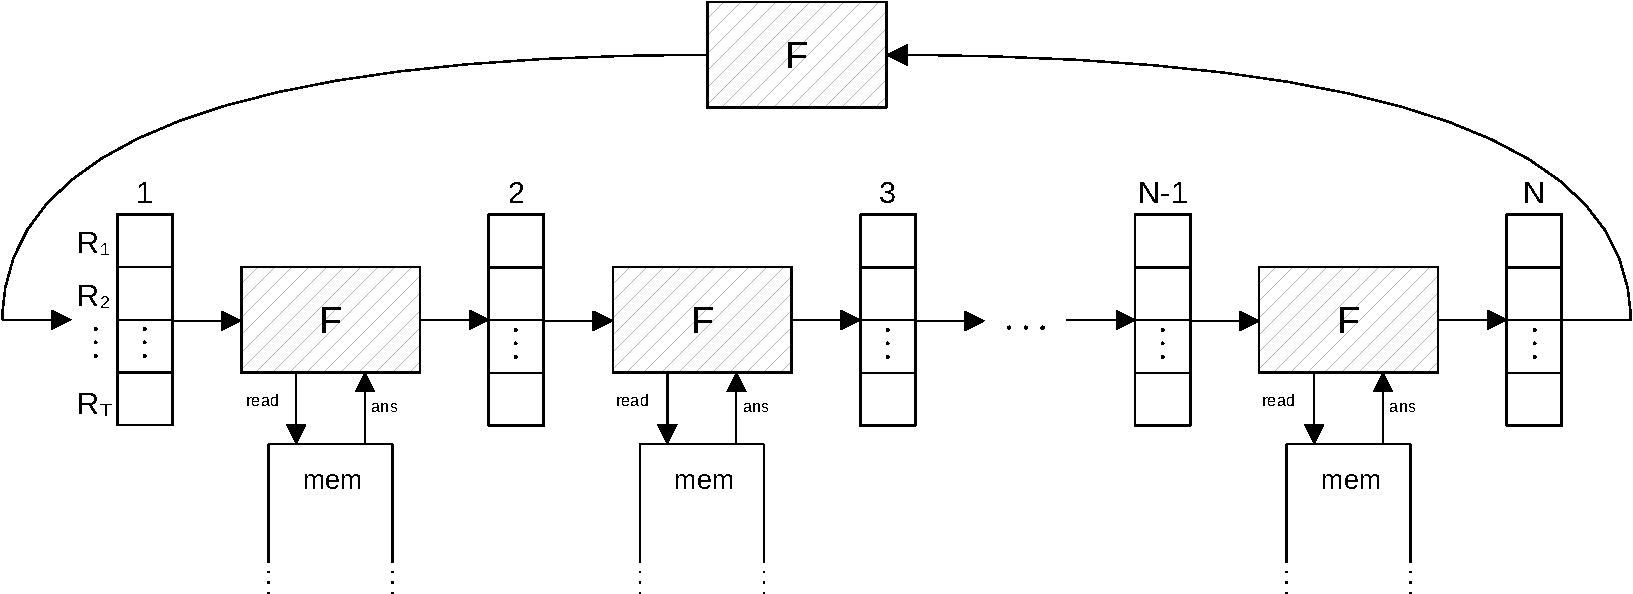
\includegraphics[width=0.8\textwidth]{../figures/computation-memory-diagram}
    \caption{Depiction of our model with $T$ registers and $N$ steps.}
    \label{fig:comp-model}
\end{figure}

Specifically, our model is parameterized by two positive integers $(T, N)$, one representing the number of registers and the other representing the number of steps, and it consists of the following components:
\begin{enumerate}
    \item \textit{Registers}. A constant number $T$ of \textit{registers} $R_1,\dots,R_T$. Registers are a set of accessible cells that are available and can be manipulated by our machine in each state transition. Each of them contains data that, unless stated otherwise, is represented by an element in $\FF$. We use $r_{i,j}$ to denote the field element that, at step $i$, is contained in register $R_j$, with $i\in[N]$ and $j \in [T]$. 
    % \begin{enumerate}[a)]
        % \item \textit{Address}: A unique, distinguishable locator equivalent to a natural number.
        
        % \item \textit{Data}: Piece of information contained within a register. Unless stated otherwise, it will hold an element in $\FF$.
        % \end{enumerate}
    
    \item \textit{Memory}. Memory is the primary location from which the information is retrieved. The main difference between the memory and the registers is that while the memory cells can only store data, the registers can be manipulated by the machine. The memory is represented by an $N \times T$ matrix $\M = \{m_{i,j}\}_{i\in[N],j\in[T]}$ of field elements. At each step, the machine reads the corresponding row of $\M$ (that is, $T$ elements) by ``popping'' it off the memory and using it to compute the next step. 
    \begin{remark}
        Notice that since our machine is read-only, the elements that are read from memory are never ``pushed'' back.
    \end{remark}
    
    % \item \textit{The Program Counter}. Every register machine will contain a special register called the program counter (PC), which tells the machine what is the next instruction to execute.
    
    \item \textit{State Transition Function}. As mentioned before, the \textit{state} of a machine at a given point $i$ consists of the set of $T$ elements from $\FF$ that its registers hold at the $i$-th step of the computation. The machine defines a state transition function $f \colon \FF^{2T} \to \FF^T$ that updates the $i$-th state to the $(i+1)$-th state having as input both the $i$-th state and the data stored in the memory. More concretely, for each step $i \in [N-1]$, the function $f$ satisfies:
    \[
    f(r_{i,1},\dots,r_{i,T},m_{i,1},\dots,m_{i,T}) = (r_{i+1,1},\dots,r_{i+1,T}),
    \]
    and for $i = N$:
    \[
    f(r_{N,1},\dots,r_{N,T},m_{N,1},\dots,m_{N,T}) = (r_{1,1},\dots,r_{1,T}),
    \]
    i.e., $f$ ensures that the state evolves correctly and that it ``cycles back'' from the last state to the first one.
    
    \begin{remark}
        This cyclic relation avoids the need of defining the common notions of inputs and outputs in our model. Moreover, the ordering of our model's states can be shifted in any number of positions and in both directions, so that when we refer to a first or last state we assume that an ordering has been previously fixed.
    \end{remark}
\end{enumerate}

% In the following we refer to the \textit{front-end} of our model as the process of converting a computer program into its equivalent description in terms of our model. More specifically, given a program

\begin{definition}[Arithmetic Circuit]
    An \textit{arithmetic circuit $C$} over a field $\FF$ is a directed acyclic graph in which input and output nodes are connected with intermediate nodes through wires. The nodes are typically called \textit{gates} and are labeled by either $+$ (a \textit{sum} gate) or $\times$ (a \textit{product} gate), with two exceptions. First, every node in it with in-degree zero is called an \textit{input gate} and is labeled by either a variable $x_i$ or an element from $\FF$. Second, every node in it with outdegree zero is called an \textit{output gate} and is labeled by a polynomial with coefficients from $\FF$.
    
    The AC processes its input, hence obtaining a polynomial, in the following way. Starting from the input gates, their path is followed and in the process, some gates compute the sum of the polynomials computed by their children, while product gates compute the product of the polynomials computed by their children. A simple example of this process is illustrated in Fig. \ref{fig:arithmeticCircuit}.
\end{definition}

\begin{figure}[H]
    \centering
    \begin{tikzpicture}
        % vertices
        \node[vertex] (1) at  (0,0) {$+$};
        \node[below left=0.5cm of 1, vertex, fill=cyan!20!white] (A) {$x_1$};
        \node[below right=0.5cm of 1, vertex, fill=cyan!20!white] (B) {$x_2$};
        \node[vertex] (2) at  (2,0) {$\times$};
        \node[right=1.4cm of 2,,yshift=15pt] (F) {Intermediate Gates};
        \node[below right=0.5cm of 2, vertex, fill=cyan!20!white] (C) {$11$};
        \node[right=0.5cm of C] (E) {Input Gates};
        \node[vertex] (3) at  (1,1) {$+$};
        \node[above=0.5cm of 3, rectangle, draw] (D) {$(x_1 + x_2) + 11 \cdot x_2$};
        \node[right=1cm of D] (G) {Output Gates};
        %edges
        \draw[edge] (A) to node[left,xshift=2pt,yshift=4pt]{} (1);
        \draw[edge] (B) to node[right,xshift=0pt,yshift=4pt]{} (1);
        \draw[edge] (B) to node[left,xshift=0pt,yshift=4pt]{} (2);
        \draw[edge] (C) to node[right,xshift=0pt,yshift=4pt]{} (2);
        \draw[edge] (1) to node[right,xshift=0pt,yshift=4pt]{} (3);
        \draw[edge] (2) to node[right,xshift=0pt,yshift=4pt]{} (3);
        \draw[edge] (3) to node[left,xshift=0pt,yshift=4pt]{} (D);
    \end{tikzpicture}
    \caption{Arithmetic circuit that performs two additions and one multiplication.}
    \label{fig:arithmeticCircuit}
\end{figure}


%%%%%%%%%%%%%%%%%%%%%%%%%%%%%%%%%%%%%%%%%%%%%%%%%%%%%%%%%%%%%%%%%%%%%%%%%%%%%%%%
\subsection{Arithmetization: The Bridge Between PIL and our Model}

\begin{table}[H]
    \centering
    \begin{tabular}{|c|l|}
        \hline
        \textbf{PIL Keyword} & \textbf{Register Machine Equivalent} \\\hline
        \tt{namespace} & Defines a new machine. \\\hline
        \tt{pol commit} & Creates a new register. \\\hline
        \tt{pol const} &  \\\hline
        \tt{=} & Defines (a part of) the state transition function. \\\hline
        \tt{pol} &  \\\hline
        \tt{public} &  \\\hline
    \end{tabular}
    \caption{TBD}
    \label{fig:TBD}
\end{table}

In this section, we introduce the basic keywords used in PIL and how they relate to our model. The starting point is the process of \textit{arithmetization} of our model. This means that to arithmetize our model, we must specify the transition function $f$ as a set of polynomial constraints over variables representing the \enquote{current} and the \enquote{next} step of the state.

\begin{definition}[Arithmetization]
    Let $\bar{X}$ be a shorthand for the sequence of formal variables $X_1,\dots, X_T$, $\bar{M}$ a shorthand for the sequence of formal variables $M_1,\dots, M_T$ and $\bar{Y}$ a shorthand for the sequence of formal variables $Y_1\dots, Y_T$. Given a state transition function $f \colon \FF^{2T} \to \FF^T$, the \textit{arithmetization of $f$} consists on computing polynomials $p_1,\dots,p_T \in \FF[\bar{X},\bar{M},\bar{Y}]$ such that for each input state $x \in \FF^{T}$, memory row $m \in \FF^T$ and next state $y \in \FF^T$, we have that:
    \[
    f(x,m) = y \quad \text{ if and only if } \quad p_i(x,m,y) = 0 \text{ for all } i \in [T].	
    \]
    % The aritmetization will be considered to be correct if, given a pair of input $x\in \FF^{2T}$ and output $y \in \FF^T$, we have that $f(x)=y$ if and only if the polynomial constraints get satisfied on this pair.
\end{definition}


% \begin{definition}[execution trace]
    %     The \textit{execution trace} of our model is the matrix of $N \times T$ field elements where:
    %     \begin{enumerate}
        %     \item Each row $i \in [N]$ corresponds with the state of the machine at the $i$-th step.
        
        %     \item Each column $j \in [T]$ corresponds with the content of the $j$-th register over every step.
        %     \end{enumerate}
    % \end{definition}




%%%%%%%%%%%%%%%%%%%%%%%%%%%%%%%%%%%%%%%%%%%%%%%%%%%%%%%%%%%%%%%%%%%%%%%%%%%%%%%%
\subsection{Register Machine Relation}



%%%%%%%%%%%%%%%%%%%%%%%%%%%%%%%%%%%%%%%%%%%%%%%%%%%%%%%%%%%%%%%
\subsection{Related Work}

The main objective of STARK-based languages is translating a computation described as a computer program to a computation described as an AIR. The distinct ways this process can be achieved can be divided into two:
\begin{enumerate}
    \item \textbf{ASIC-like}: This approach is based on writing a computer program in some domain-specific language (DSL) that compiles to an equivalent AIR representing the satisfiability of the computer program. Examples of such are PIL itself and AirScript \cite{AirScript}.
    \item \textbf{CPU-like}: This approach attempts to design an AIR that behaves like a CPU that can handle any computation passed to it. This means that a program is no longer directly compiled into AIR. Instead, the program is compiled to a reduced set of assembly instructions that are understood by the CPU and then the assembly program is transformed to the single AIR representing the correct execution of the CPU. Examples of such are Zilch \cite{EPRINT:MouTso20} and Cairo \cite{EPRINT:GolPapRia21}.
\end{enumerate}

None of the previous variants is the best for every computer program we can think of, as they present several advantages and disadvantages depending on the particular program they are dealing with. Even if more involved, we preferred the ASIC-like approach for PIL for the following reasons:
\begin{enumerate}[a)]
    \item Efficiency: Since the AIR is dependent on the specific computer program, one can design an AIR tailored to that program. In particular, one can decide whether his design is based on a ``wider'' and ``shorter'' or on a ``thinner'' and ``higher'' execution trace.
    \item Modularity: One can divide a program into multiple small pieces (relating these pieces appropriately) and produce an AIR for each piece separately that will ultimately produce an AIR for the entire program. This allows the user to build a vast program through handle (small) logic. 
\end{enumerate}

Similar to PIL, AirScript is a DSL to produce AIR constraints in an ASIC-like fashion. The main problem of AirScript is that it has very little abstraction for describing non-identity constraints. While PIL has built-in keywords for such constraints (that could be augmented in the future), an AirScript user needs to deal with them explicitly: for any argument that is based on random field elements supplied by the verifier during the protocol, a user must define identity constraints attesting the argument's validity by accessing the verifier's randomness. For example, if one wants to produce a program checking that a column is a value in the range $[0,2^4-1]$ by using the Plookup \cite{EPRINT:GabWil20} inclusion argument (in the style described in \cite{EPRINT:PFMBM22}):
\begin{pil}
    namespace Example();
    pol commit a;
    pol constant BITS4;
    
    a in BITS4;
\end{pil}
\begin{pil}
    def Example
    trace_columns:
    main: [a,BITS4,h1,h2]
    aux: [Z]
    
    boundary_constraints:
    enf Z.first = 1
    
    integrity_constraints:
    enf Z'*($rand[0]*(1+$rand[1])+h1+$rand[1]*h2)*($rand[0]*(1+$rand[1])+h2+$rand[1]*h1') = Z*(1+$rand[0])*($rand[1]+a)*($rand[0]*(1+$rand[1])+BITS4+$rand[1]*BITS4')
\end{pil}
Even tho more generic, an AirScript user must choose and understand the argument he wants to deal with, making it less attractive than PIL to the public. 

Regarding CPU-like approaches like Zilch and Cairo, they are both based on a similar workflow: (1) write a program for the computation (either using an assembly-like language directly or using any other language that can be compiled to the CPU bytecode); (2) compile the program to the CPU bytecode; and (3) use a STARK prover for the single AIR to generate a proof. This two-step paradigm suffers from efficiency, as the set of assembly instructions is unlikely to be optimal for every single program. Therefore, while step (3) is independent of the specific program that the user deals with (something that appears to be very handy in proof systems), this does not justify the overhead generated in step (2) as vast programs might have an untractable bytecode whose proof might take too long to compute for practical deployment.



\section{Our Techniques}

In this section we explain the main differences between the techniques used during the rounds of the vanilla STARK (Section \ref{sec:vanilla-STARK}) and our techniques. 


%%%%%%%%%%%%%%%%%%%%%%%%%%%%%%%%%%%%%%%%%%%%%%%%%%%%%%%%%%%%%%%
\subsection{Commiting to Multiple Polynomial at Once}\label{sec:committing}

For this section, explicitly set $H = \{h_1,h_2,h_3,\dots,h_m\}$.
% , where $h \in \FF$ is an element of order $2^kn$, with $2^k$ typically called the \textit{blowup factor}, and $s \in \FF\backslash H$ is a field element chosen to obtain such coset.From now on we will denote by $m$ to $2^kn$ for notation clarity. 
% In this section it will be important to keep in mind that the characterisitic of the field chosen to be $2^{64} - 2^{32} + 1$.
Also, denote by $f_0,f_1,\dots,f_N \in \FF_{<n}[X]$ the set of polynomials that we want to construct the Merkle Tree on. That is, the input to the Merkle Tree constructor is the set of evaluations:
\[
\begin{array}{|ccccc|}
\hline
f_0(h_1), & f_1(h_1), & f_2(h_1), &\dots, &f_N(h_1) \\[0.1cm]
f_0(h_2), & f_1(h_2), & f_2(h_2), &\dots, &f_N(h_2) \\
\vdots & \vdots &\vdots &\cdots & \vdots \\
f_0(h_m), & f_1(h_m), & f_2(h_m), & \dots, &f_N(h_m) \\
\hline
\end{array}
\]

A leaf element of the Merkle Tree will consist on the evaluations of all the polynomials at a single point. This will be convinient for a latter step of the STARK generation. For instance, in the batched FRI protocol we group evaluations of all the original polynomials at a common point for succinctly answering a batched consistency check. Specifically, assuming that $f_0,f_1,\dots,f_N$ are the original polynomials,  the leaf elements of the Merkle Tree, indexed by the corresponding value, will consist on:
\[
\begin{array}{|ccc|}
\hline
\text{leaf } h_1 & \Longrightarrow & \H(f_0(h_1), f_1(h_1), f_2(h_1), \dots, f_N(h_1)) \\[0.1cm]
\text{leaf } h_2 & \Longrightarrow & \H(f_0(h_2), f_1(h_2), f_2(h_2), \dots, f_N(h_2)) \\
\vdots &  & \vdots \\[0.1cm]
\text{leaf } h_m & \Longrightarrow & \H(f_0(h_m), f_1(h_m), f_2(h_m), \dots, f_N(h_m)) \\
\hline
\end{array}
\]
where $\H$ is any collision resistant hash function. Notice how if $h_i$ is the requested point of check by the verifier, then the prover can prove the consistency of all the evaluations $f_0(h_i),\dots,f_N(h_i)$ with the corresponding Merkle root in a single Merkle path.

%TODO: Be sure it satisfies round-by-round soundness.....
A proof that the resulting non-interactive protocol is knowledge sound after applying the Fiat-Shamir using this strategy can be found, for example, in Theorem 4 of \cite{EPRINT:AttFehKlo21}.


\ifPOLYGON
To be more specific, the hash function $H$ is set to be the Poseidon \cite{USENIX:GKRRS21} hash function. Poseidon was chosen because it was created to minimize prover and verifier complexities when zero-knowledge proofs are generated and validated. Notably, the best hashing performance is obtained when the state size is limited to $12$ field elements, $4$ of which are occupied by the capacity of the hash function. This implies that, in order to get the best Poseidon performance, we have to restrict the input size to be of $8$ field elements.

Leaf hashes are performed ``linearly''. By linearly we mean that, if the input to the hash function is $t_1(sh^i)$, $t_2(sh^i)$, $\dots$, $t_N(sh^i)$, then we process it as follows:
\begin{enumerate}
	\item The input is split in chunks of $8$ elements, filling with repetitions of the $0$ element if $N$ is not a multiple of $8$.
	\item The first chunk is hashed using Poseidon with capacity $(0, 0, 0, 0)$.
	\item The following chunk is hashed using Poseidon with the capacity being the output of the previous hash.
	\item Go to Step 3 until there are no more chunks.
\end{enumerate}

An example of this process can be seen in the Figure \ref{fig:linear-hash}.
\begin{figure}[H]
	\centering
	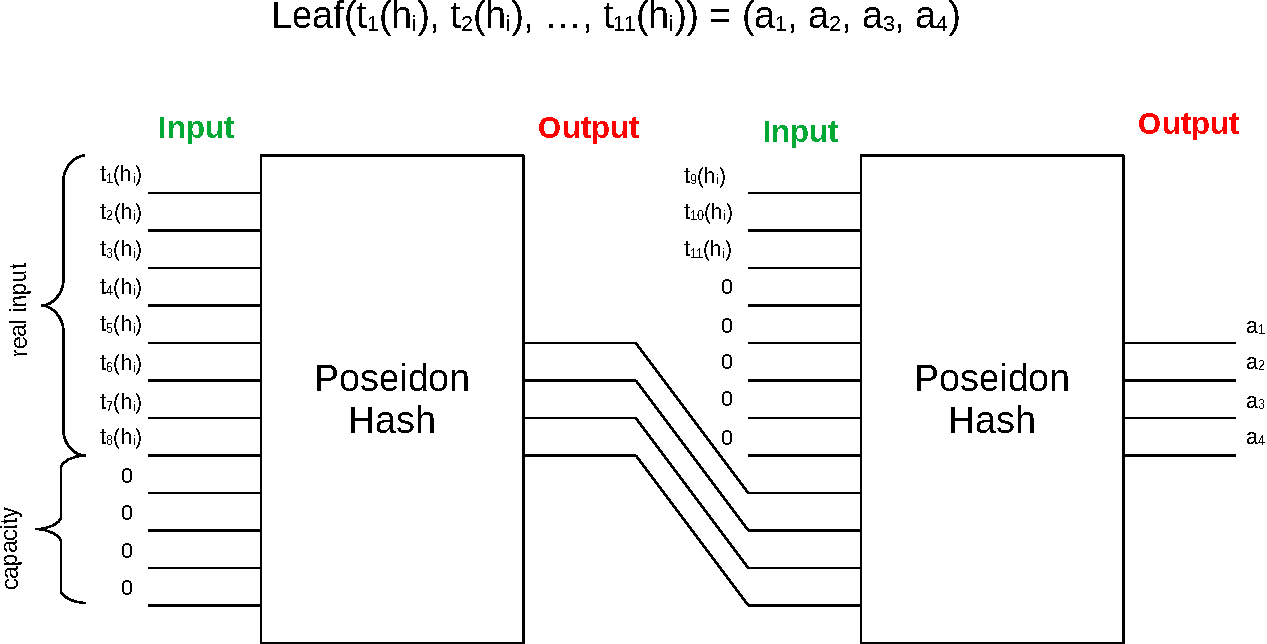
\includegraphics[width=.7\textwidth]{../figures/poseidon-linear-hash}
	\caption{Leaf hash computation on input $(t_1(sh^i), \dots, t_{11}(sh^i))$ in a linear manner.}
	\label{fig:linear-hash}
\end{figure}

Once all the hashed leafs are obtained, one starts to construct the Merkle tree by continually hashing two child nodes using Poseidon with capacity $(0,0,0,0)$ and defining the parent node as the output. This that this is well defined because Poseidon's output consist on $4$ field elements, while its input size consists on $8$. See Figure \ref{fig:full-poseidon} for an example with $4$ leafs.
\begin{figure}[H]
	\centering
	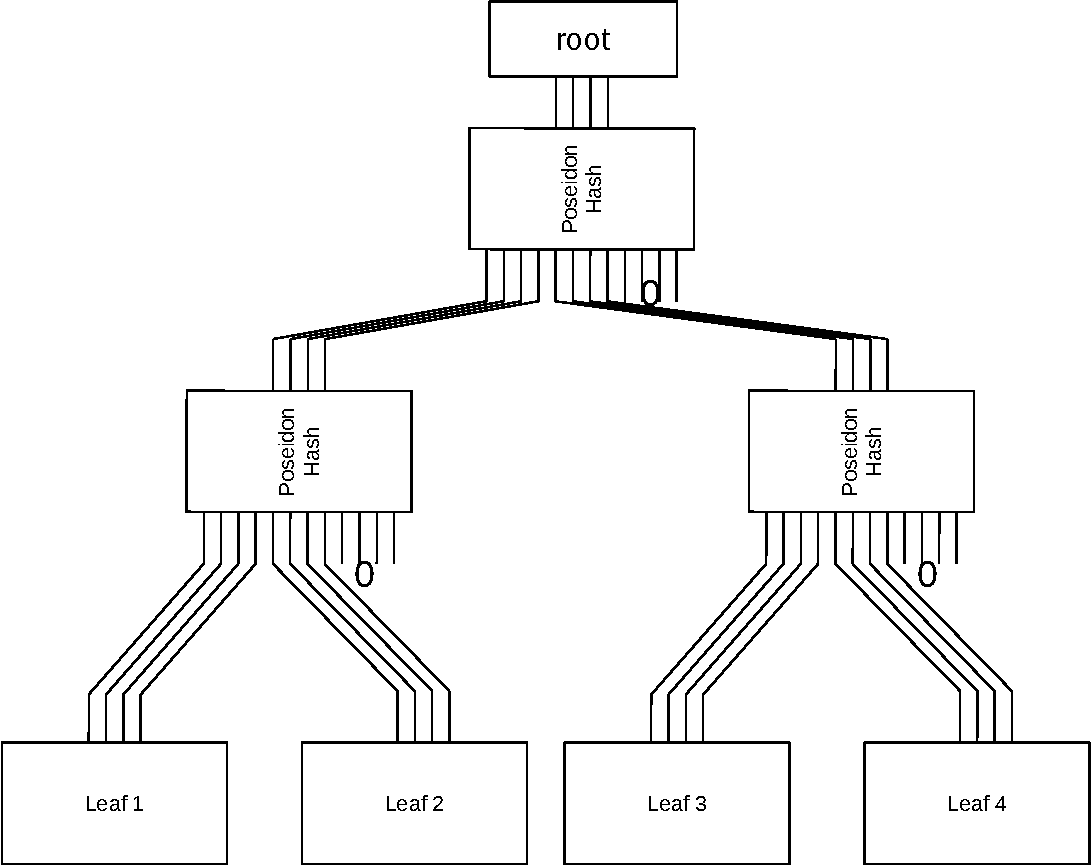
\includegraphics[width=.6\textwidth]{../figures/MT-poseidon-example}
	\caption{Merkle's tree hash computation assuming $4$ leafs.}
	\label{fig:full-poseidon}
\end{figure}

In fact, this procedure has been extended in order to being able to compute hashes faster using several GPUs. First of all, we are splitting all our polynomials in $4$ chunks of size:
\[
\mathtt{batchSize} = \Biggl\lfloor \max \left( 8, \frac{N + 3}{4} \right)  \Biggr\rfloor.
\]

Of course, it may be possible that not all of the chunks have exactly this amount of elements. In this case, we prioritize to fill the first $3$ ones up to this size, letting the last one become smaller, but not so smaller. The idea is that, with the formula above, the chunk size is increased by $1$ once $N$ increase by $4$ (when $N > 32$, which is the first time when all chunks has exactly \texttt{batchSize} number of elements). Hence, for $N$ big enough, the last chunk never will become smaller than $\mathtt{batchSize} - 3$, becoming a almost uniform distribution of the polynomials among the $4$ chunks. Table \ref{tab:multi-gpu-chunks} shows several examples on how this chunk division sizes looks like.

\begin{figure}[h!]
	\centering
	\[
	\begin{array}{|c|c|c|c|c|c|}
	\hline
	N	&\texttt{batchSize}	&\textbf{Chunk 1}	&\textbf{Chunk 2}	&\textbf{Chunk 3}	&\textbf{Chunk 4}	\\
	\hline
	1		&8			&1				&0				&0				&0				\\
	\cdots	&\cdots		&\cdots			&\cdots			&\cdots			&\cdots			\\
	8		&8			&8				&0				&0				&0				\\
	9		&8			&8				&1				&0				&0				\\
	10		&8			&8				&2				&0				&0				\\
	\cdots	&\cdots     &\cdots			&\cdots			&\cdots			&\cdots			\\
	17		&8			&8				&8				&1				&0				\\
	\cdots	&\cdots		&\cdots			&\cdots			&\cdots			&\cdots			\\
	25		&8			&8				&8				&8				&1				\\
	\cdots	&\cdots		&\cdots			&\cdots			&\cdots			&\cdots			\\
	32		&8			&8				&8				&8				&8				\\
	33		&9			&9				&9				&9				&6				\\
	34		&9			&9				&9				&9				&7				\\
	35		&9			&9				&9				&9				&8				\\
	36		&9			&9				&9				&9				&9				\\
	37		&10			&10				&10				&10				&7				\\
	38		&10			&10				&10				&10				&8				\\
	\cdots	&\cdots		&\cdots			&\cdots			&\cdots			&\cdots			\\
	51		&13			&13				&13				&13				&12				\\
	\cdots	&\cdots		&\cdots			&\cdots			&\cdots			&\cdots			\\
	\hline
	\end{array}
	\]
	\caption{Chunk's size distribution for several values of $N$.}
	\label{tab:multi-gpu-chunks}
\end{figure}

After the polynomial splitting in $4$ chunks (say $T_1, T_2, T_3$ and $T_4$), we perform the previously defined linear hash of all of them in a parallel way, ending up with a set of a maximum amount of $16$ field elements corresponding to the $4$ outputs of $4$ field elements each. To finish this updated version of the linear hash, we perform the linear hash of this $16$ elements as done previously, which outputs a final total amount of $4$ field elements. More precisely, if 
\[
LH(T_i) = (H_{i, 1}, H_{i, 2}, H_{i, 3}, H_{i, 4})	\quad i \in \{1, 2, 3, 4\},
\]
then the final output will be
\[
\scalebox{0.85}{\mbox{\ensuremath{\displaystyle 
			LH(H_{1, 1}, H_{1, 2}, H_{1, 3}, H_{1, 4}, H_{2, 1}, H_{2, 2}, H_{2, 3}, H_{2, 4}, H_{3, 1}, H_{3, 2}, H_{3, 3}, H_{3, 4}, H_{4, 1}, H_{4, 2}, H_{4, 3}, H_{4, 4})
}}},
\]
where $LH$ denotes the single-GPU version of the linear hash. 



\subsection{Transcript Generation and Computing Verifier Challenges}\label{sec:transcript-gen}

We will describe our protocol version as a non-interactive protocol using the Fiat-Shamir heuristic \cite{C:FiaSha86}. Therefore, we need to specify how we are generating the random challenges from $\KK$ (or equivalently, $3$ elements of $\FF$). Through all this section we will use an instance of a Poseidon hash function having state size of $12$ field elements ($8$ for inputs and $4$ for capacity) and output size of $12$ field elements. 

The strategy for generating the transcript is similar to the linear hash strategy described before. Suppose we want to add $c_1, \dots, c_r$ elements to the transcript. We proceed as follows:

\begin{enumerate}

\item The input is split in chinks of $8$ field elements, filling with repetitions of the $0$ element if $r$ is not a multiple of $8$. 

\item The first chunk is hashed using Poseidon with capacity $(0,0,0,0)$.

\item The following chunk is hashed using Poseidon with the capacity being the $4$ last elements of the output of the previous hash. 

\item Go to Step $3$ until there are no more chunks. 

\end{enumerate}

Observe that the $8$ remaining elements of each hash output are not being used until we stop the loop between the steps $3$ and $4$. We depict the previous strategy in Figure \ref{fig:transcript-gen}.  

\begin{figure}[h!]
\centering
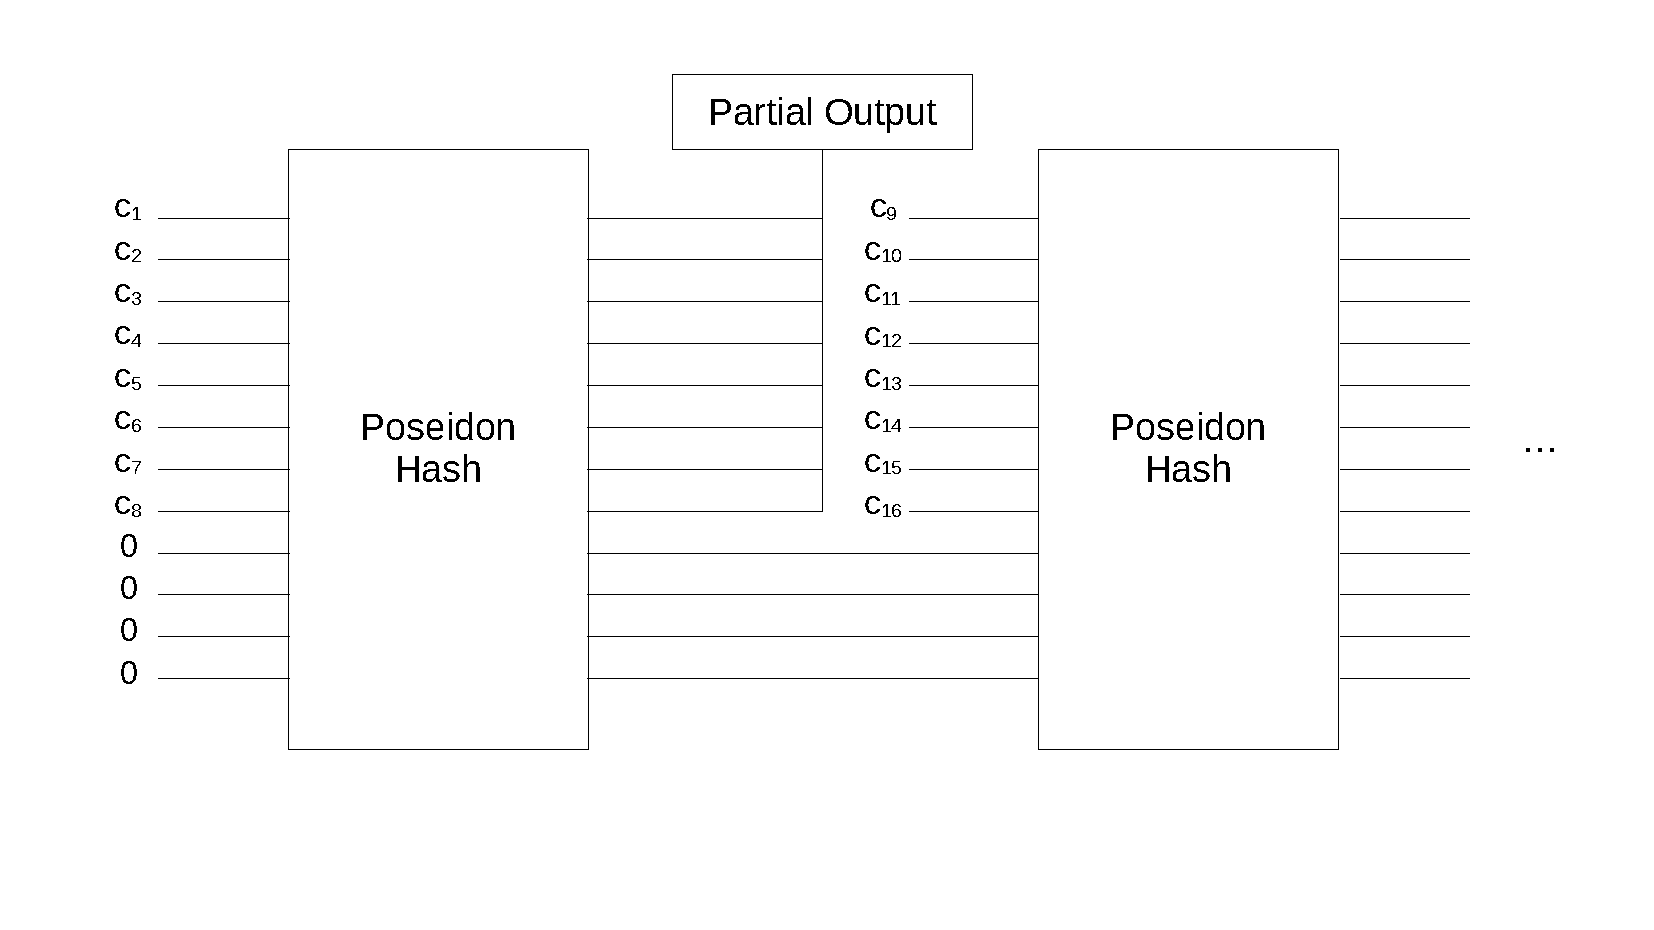
\includegraphics[width=.8\textwidth]{../figures/transcript}
\caption{First two steps of the transcript generation.}
\label{fig:transcript-gen}
\end{figure}

When we stop adding elements to the transcript, we end up with an output consisting in $8$ field elements, say $(t_1, \dots, t_8)$. For a given transcript state we can extract at most $3$ challenges of $\KK$. The first two elements are trivially obtained
\[
t_1 + t_2 \varphi + t_3 \varphi^2, \quad t_4 + t_5 \varphi + t_6 \varphi^2
\]
for $\varphi$ being a root of the irreducible polynomial used to construct $\KK$ from $\FF$. Since we do not have enough elements to construct a third extension field element, we proceed as follows. We construct an field element $t_9$ hashing $8$ zeros with the capacity being the last $4$ output elements of the last hash performed at the time of generating the transcript (that is, the elements that will become the capacity of the next hash when adding a new element into the transcript). Hence, we get a third element in $\KK$
\[
t_7 + t_8 \varphi + t_9 \varphi^2.
\]
However, observe that we can not extract more than that. 

We will denote by \transcript the transcript instance and we will define for it the following operations:

\begin{itemize}

\item \textbf{Add:} Having elements $c_1, \dots, c_r \in \FF$, we denote by 
\[
\transcriptAdd(c_1, \dots, c_r)
\]
the operation of adding $c_1, \dots, c_r$ to the transcript using the previous procedure. 

\item \textbf{Extract:} Having a transcript state \textsf{T}, we denote by
\[
\transcriptExtract{i}(\transcript) \in \KK \quad i \in \{1, 2, 3\}
\]
the result of extracting a single extension field $\KK$ element from it using the previously described procedure. Using the notation above:
\begin{align*}
&\transcriptExtract{1}(\transcript) = t_1 + t_2 \varphi + t_3 \varphi^2, \\
&\transcriptExtract{2}(\transcript) = t_4 + t_5 \varphi + t_6 \varphi^2, \\
&\transcriptExtract{3}(\transcript) = t_7 + t_8 \varphi + t_9 \varphi^2.
\end{align*}
\end{itemize}

A proof that the resulting non-interactive protocol is knowledge sound after applying the Fiat-Shamir using this strategy can be found, for example, in Theorem 4 of \cite{EPRINT:AttFehKlo21}.

\fi



%%%%%%%%%%%%%%%%%%%%%%%%%%%%%%%%%%%%%%%%%%%%%%%%%%%%%%%%%%%%%%%
\subsection{Preprocessed Polynomials and Public Values}\label{sec:preprocessed-public}

Among the set of polynomials that are part of the polynomial constraint system representing the problem's statement, we differentiate between two types: \textit{committed polynomials} and \textit{preprocessed polynomials}. 

Committed polynomals are those polynomials for which the verifier only has oracle access and are therefore committed (via Merkle trees) by the prover before the verifier starts querying them. In other words, these polynomals can only be known, in principle, in its entire form by the prover of the protocol. Constrastly, the verifier is limited to know a ``small fraction'' of these polynomials' coefficients. In practise, this fraction is randomly chosen by the verifier and is proportional to the number of oracle queries that the verifier makes to the particular polynoial. For the shake of the protocols to be scalable, the number of queries made to committed polynomials should be at most logarithmic in their degree. An example of committed polynomials are trace columns polynomials $\tr_i$.

On the other hand, preprocessed polynomials are totally known by the verifier even before the execution of the corresponding protocol. More precisely, once a polynomial constraint system $\C$ is fixed, the verifier has complete access (either in coefficient form or in evaluation form) to the set of preprocessed polynomials. As with committed polynomials, the verifier ends up needing only a small subset of evaluations of such polynomials. An example of preprocessed polynomials are Lagrange polynomials $L_i$.

\begin{example}\label{example:pre-public}
  As an example, the polynomial constraint such that for all $x\in G$ satisfies:
  \begin{equation}\label{eq:pre-public}
    L_1(x) (\tr_1(x) - 7) = 0,
  \end{equation}
  is composed of the committed polynomial $\tr_1$ and the preprocessed (Lagrange) polynomial $L_1$, and is satisfied if and only if $\tr_1(g) = 7$.  
\end{example}


Finally, \textit{public values} are defined as the set of committed polynomials evaluations that are attested by some constraint. Clearly, public values are known to both the prover and the verifier and a particular polynomial can have many public values associated with it. In Example \ref{example:pre-public}, the value $\tr_1(g)$ is a public value since Eq. \eqref{eq:pre-public} constraints it to be equal to $7$. 


%TODO: Write this section with different degrees in both sides
%%%%%%%%%%%%%%%%%%%%%%%%%%%%%%%%%%%%%%%%%%%%%%%%%%%%%%%%%%%%%%%
\subsection{Adding Selected Vector Arguments}\label{sec:vector-arguments}

In this section, we describe how to augment the type of available constraints
with the arguments presented in Section \ref{sec:preliminaries:arguments}.
Recall that we will add three new types of arguments:
\begin{itemize}
  \item \textbf{Lookup ($\in$)}. The set constructed from the evaluations of a polynomial $f$ over a multiplicative subgroup $G$ is contained in an equally defined set of another polynomial $t$. We denote it as $f \in t$.
  \item \textbf{Multiset Equality ($\doteq$)}. The vector constructed from the evaluations of a polynomial $f$ over a multiplicative subgroup $G$ is a permutation of an equally defined vector of another polynomial $t$. We denote it as $f \doteq t$.
  \item \textbf{Connection ($\propto$)}. The vector constructed from the evaluations of a set of polynomials $f_1,\dots,f_{\ell}$ over a multiplicative subgroup $G$ does not vary after applying a known permutation $\sigma$ to them. We denote it as $(f^{(1)},\dots,f^{(\ell)} \propto (S^{(\sigma_1)},\dots,S^{(\sigma_{\ell})})$.
\end{itemize}
In order to include non-identity constraints to the protocol, we will represent them through their succinct set of identity constraints. We denote by $M^{\in}$ the number of lookup instantiations, $M^{\doteq}$ the number of multiset equality instantiations and $M^{\propto}$ the number of connection instantiations.

As detailed in Section \ref{sec:preliminaries:arguments}, for the 
lookup argument, we need to compute and commit the associated polynomials $h_{1,j}$ and $h_{2,j}$ before being able to compute the corresponding grand-product polynomial for each lookup constraint $j \in [M]$. 
This sums up to $2M$ polynomials.
After this, for each non-identity constraint, we compute the associate grand-product polynomial $Z$ and commit to it. This definition of this polynomial is different depending on which argument we are executing as
shown in Section \ref{sec:preliminaries:arguments}.
This sums up to $M$ lookup polynomials, $M'$ multiset equality polynomials and $M''$ connection polynomials. Overall, adding non-identity constraints adds up to $3M + M' + M''$ polynomials (that will need to be committed) and $2(M+M'+M'')$ polynomial constraints to the STARK.
%TODO: Check if the number of polynomials in the connection argument can be reduced to one somehow, similar to lookups and permutations (as I explain in the following section).

%TODO: Motivate it with examples? Not necessary

Following, we explain how we generalize both lookups and multiset equalities to not only involving multiple polynomials, but also to a subset of the resulting vector. Therefore, somewhat artificially, enlarge the expressiveness of our arguments and let us handle more generic non-identity constraints.
% Let's explain first how we reduce vector lookups or multiset equalities to simple (i.e., one polynomial) lookups or multiset equalities.
% \begin{definition}[Vector Arguments]
%   Given $2R$ multivariate polynomials $C_i \in \FF[X_1,\dots,X_N]$ and $N$ univariate polynomials $P_i \in \FF[X]$, a \textit{vector lookup} is the argument in which for all $x \in G$ there exists some $y \in G$ such that:
%   \begin{equation}\label{eq:vector-lookup}
%     ((C_1 \circ \otr)(x),\dots,(C_R \circ \otr)(x)) = ((C_{R+1} \circ \otr)(y),\dots,(C_{2R} \circ \otr)(y)).
%   \end{equation}
%
%   A \textit{vector permutation} is defined analogously, but multiplicies of elements should be the same. That is, if for instance there exists $x_1,x_2 \in G$ such that $(C_1 \circ \otr)(x_1),\dots,(C_R \circ \otr)(x_1) = (C_1 \circ \otr)(x_2),\dots,(C_R \circ \otr)(x_2)$, then there should exist $y_1,y_2 \in G$ such that $(C_{R+1} \circ \otr)(y_1),\dots,(C_{2R} \circ \otr)(y_1) = (C_{R+1} \circ \otr)(y_2),\dots,(C_{2R} \circ \otr)(y_2)$ and for which Eq. \eqref{eq:vector-lookup} holds.
% \end{definition}
%
% To reduce the previous vector argments to simple ones, we make use of a uniformly sampled element $\alpha \in \KK$. Namely, instead of trying to generate a grand-product polynomial for Eq. \eqref{eq:vector-lookup}, we define the following polynomials:
% \begin{align}\label{eq:vector-simple}
% \begin{split}
%   F'(X) &:= (C_1 \circ \otr)(X) + \alpha (C_2 \circ \otr)(X) + \dots +\alpha^{R-1}(C_R \circ \otr)(X), \\[0.1cm]
%   T'(X) &:= (C_{R+1} \circ \otr)(X) + \alpha (C_{R+2} \circ \otr)(X) + \dots + \alpha^{R-1}(C_{2R} \circ \otr)(X),
% \end{split}
% \end{align}
% and compute the grand-product polynomial for the relation $F' \in T'$ or $F' \doteq T'$. Notice that both $F'$ and $T'$ are in general polynomials with coefficients over the field extension $\KK$. This reduction leads to the following result, whose proof is a direct consequence of the Schwartz–Zippel lemma.
%
% \begin{lemma}\label{col:vector-to-simple}
%   Given $F',T' \in \KK[X]$ as defined by Eq. \eqref{eq:vector-simple}, if $F' \in T'$, then Eq. \eqref{eq:vector-lookup} (respectively the equation for vector permutations) holds excepts with probability $n \cdot R/|\KK|$ over the random election of $\alpha$.
% \end{lemma}
%
% Now, let's go one step further by the introduction of \textit{selectors}. Informally speaking, a selected lookup (permutation) is a lookup (permutation) not between the specified two polynomials $f,t$, but between the polynomials generated by the multiplication of $f$ and $t$ with (generally speaking) independently generated selectors. We generalize to the vector setting.
% \begin{definition}[Selected Vector Arguments]\label{def:sel-args}
%   We are given $2R$ multivariate polynomials $C_i \in \FF[X_1,\dots,X_N]$ and $N$ univariate polynomials $P_i \in \FF[X]$. We are also given two polynomials $\fsel,\tsel \in \FF[X]$ whose range over the domain $G$ is $\{0,1\}$. That is, $\fsel$ and $\tsel$ are \textit{selectors}. A \textit{selected vector lookup} is the argument in which for all $x \in G$ there exists some $y \in G$ such that:
%   \begin{equation}\label{eq:selected-lookup}
%     \fsel(x) \cdot  ((C_1 \circ \otr)(x),\dots,(C_R \circ \otr)(x)) = \tsel(y) \cdot ((C_{R+1} \circ \otr)(y),\dots,(C_{2R} \circ \otr)(y)).
%   \end{equation}
%
%   A \textit{selected vector permutation} is defined analogously, but multiplicies of elements should be the same. 
% \end{definition}
%
% \begin{bremark}
% Note that if $\fsel = \tsel = 1$, then Eq. \eqref{eq:selected-lookup} is reduced to \eqref{eq:vector-lookup}; if $\fsel = \tsel = 0$ then the argument is trivial; and if either $\fsel$ or $\tsel$ are equal to the constant $1$, then we remove the need for $\fsel$ or $\tsel$, respectively.
% \end{bremark}
%
% To reduce the previous selected vector lookup to simple ones, we proceed in two steps. First, we use the reduction in Eq. \eqref{eq:vector-simple} to reduce the inner vector argument to a simple one. This process outputs polynomials $F',T' \in \KK[X]$. Second, we make use of another uniformly sampled $\beta \in \KK$. Namely, instead of trying to generate a grand-product polynomial for Eq. \eqref{eq:selected-lookup}, we define the following polynomials:
% \begin{align}\label{eq:F-T-sel}
% \begin{split}
% T(X) &:= \tsel(X) [T'(X) - \beta] + \beta, \\[0.1cm]
% F(X) &:= \fsel(X) [F'(X) - T(X)] + T(X),
% \end{split}
% \end{align}
% and compute the grand-product polynomial for the relation $F \in T$. 
% Importantly, the presentation ``re-ordering'' in Eq. \eqref{eq:F-T-sel} is relevant. More precisely, if $\beta$ had been introduced in the definition of $F$ instead, then there would be situations in which we would end up having $\beta$ as a lookup value and therefore the lookup argument not being satisfied even if the selectors are correct.
% %TODO: Example of hte previous paraprah
%
% To reduce selected vector permutations to simple ones, we follow a similar process than with selected vector lookups. We also first use the reduction in Eq. \eqref{eq:vector-simple} to reduce the inner vector argument to simple one, but then we define:
% \begin{align}\label{eq:F-T-sel-perm}
%   \begin{split}
%   F(X) &:= \fsel(X) [F'(X) - \beta] + \beta,\\[0.1cm]
%   T(X) &:= \tsel(X) [T'(X) - \beta] + \beta, 
% \end{split}
% \end{align}
% Here, we have been able to firstly define $F$ since we are dealing with permutations instead of inclusions.
%
% Simlarly to the vector-to-simple reduction, we obtain the following result.
% \begin{lemma}\label{col:svector-to-simple}
%   Given $F,T \in \KK[X]$ as defined by Eq. \eqref{eq:F-T-sel} (respectively, Eq. \eqref{eq:F-T-sel-perm}), if $F \in T$, then Eq. \eqref{eq:selected-lookup} (respectively the equation for selected vector permutations) holds excepts with probability $R \cdot n/|\KK| + 1/|\KK|$ over the random (and independently) election of $\alpha$ and $\beta$.
% \end{lemma}
% \begin{proof}
%   We denote the polynomials $(C_i \circ \otr)$ by $f_i$ for $i \in [R]$, and by $t_i$ for $i > R$. Assume there exists some $x \in G$ such that for all $y \in G$ we have:
%   \[
%     \fsel(x) \cdot  (f_1(x),\dots,f_R(x)) \neq \tsel(y) \cdot (t_1(y),\dots,t_R(y)).
%   \]
%   Due to Corollary \ref{col:vector-to-simple}, we have that $\fsel(x)F'(x) = \fsel(x)(f_1(x) + \alpha f_2(x) + \dots + \alpha^{R-1} f_R(x)) \neq \tsel(y)T'(y) = \tsel(y)(t_1(y) + \alpha t_2(y) + \dots + \alpha^{R-1} t_R(y))$ except with probability $R \cdot n/|\KK|$. Therefore, we obtain:
%   \[
%     \fsel(x) [F'(x) - T(x)] + T(x) \neq \tsel(y) [T'(y) - \beta] + \beta,
%   \]
%   except with probability $1/|\KK|$.
% \end{proof}
Let's explain first how we reduce vector lookups or multiset equalities to simple (i.e., one polynomial) lookups or multiset equalities.
\begin{definition}[Vector Arguments]\label{def:vec-args}
  Given polynomials $f_i,t_i \in \KK_{<n}[X]$ for $i\in[N]$, a \textit{vector lookup} is the argument in which for all $x \in G$ there exists some $y \in G$ such that:
  \begin{equation}\label{eq:vector-lookup}
    (f_1(x),\dots,f_N(x)) = (t_1(y),\dots,t_N(y)).
  \end{equation}

  A \textit{vector mutliset equality} is defined analogously, but multiplicies of elements should be the same. That is, if for instance there exists $x_1,x_2 \in G$ such that $(f_1(x_1),\dots,f_N(x_1)) = (f_1(x_2),\dots,f_N(x_2))$, then there should exist $y_1,y_2 \in G$ such that $(t_1(y_1),\dots,t_N(y_1)) = (t_1(y_2),\dots,t_N(y_2))$ and for which Eq. \eqref{eq:vector-lookup} holds.
\end{definition}

To reduce the previous vector argments to simple ones, we make use of a uniformly sampled element $\alpha \in \KK$. Namely, instead of trying to generate a grand-product polynomial for Eq. \eqref{eq:vector-lookup}, we define the following polynomials:
\begin{align}\label{eq:vector-simple}
  F'(X) := \sum_{i=1}^N \alpha^{i-1}f_i(X), \quad T'(X) := \sum_{i=1}^N \alpha^{i-1}t_i(X),
\end{align}
and compute the grand-product polynomial for the relation $F' \in T'$ or $F' \doteq T'$. Notice that both $F'$ and $T'$ are in general polynomials with coefficients over the field extension $\KK$ even if every coefficient of $f_i,t_i$ are precisely over the base field $\FF$. This reduction leads to the following result, whose proof is a direct consequence of the Schwartz–Zippel lemma.

\begin{lemma}\label{col:vector-to-simple}
  Given polynomials $f_i,t_i \in \KK_{<n}[X]$ for $i\in[N]$ and $F',T' \in \KK_{<n}[X]$ as defined by Eq. \eqref{eq:vector-simple}, if $F' \in T'$ (resp. $F' \doteq T'$), then Eq. \eqref{eq:vector-lookup} (resp. the equation for vector multiset equality) holds excepts with probability $n \cdot (N-1)/|\KK|$ over the random election of $\alpha$.
\end{lemma}

Now, let's go one step further by the introduction of \textit{selectors}. Informally speaking, a selected lookup (mutliset equality) is a lookup (multiset equality) not between the specified two polynomials $f,t$, but between the polynomials generated by the multiplication of $f$ and $t$ with (generally speaking) independently generated selectors. We generalize to the vector setting.
\begin{definition}[Selected Vector Arguments]\label{def:sel-args}
  We are given polynomials $f_i,t_i \in \KK[X]$ for $i\in[N]$. Furthermore, we are also given two polynomials $\fsel,\tsel \in \FF[X]$ whose range over the domain $G$ is $\{0,1\}$. That is, $\fsel$ and $\tsel$ are \textit{selectors}. A \textit{selected vector lookup} is the argument in which for all $x \in G$ there exists some $y \in G$ such that:
  \begin{equation}\label{eq:selected-lookup}
    \fsel(x) \cdot  (f_1(x),\dots,f_N(x)) = \tsel(y) \cdot (t_1(y),\dots,t_N(y)).
  \end{equation}

  A \textit{selected vector multiset equality} is defined analogously, but multiplicies of elements should be the same as explained in Def. \ref{def:vec-args}.
\end{definition}

\begin{bremark}
Note that if $\fsel = \tsel = 1$, then Eq. \eqref{eq:selected-lookup} is reduced to \eqref{eq:vector-lookup}; if $\fsel = \tsel = 0$ then the argument is trivial; and if either $\fsel$ or $\tsel$ are equal to the constant $1$, then we remove the need for $\fsel$ or $\tsel$, respectively.
\end{bremark}

To reduce the previous selected vector lookup to simple ones, we proceed in two steps. First, we use the reduction in Eq. \eqref{eq:vector-simple} to reduce the inner vector argument to a simple one. This process outputs polynomials $F',T' \in \KK[X]$. Second, we make use of another uniformly sampled $\beta \in \KK$ as follows. Namely, instead of trying to generate a grand-product polynomial for Eq. \eqref{eq:selected-lookup}, we define the following polynomials:
\begin{align}\label{eq:F-T-sel}
\begin{split}
T(X) &:= \tsel(X) [T'(X) - \beta] + \beta, \\[0.1cm]
F(X) &:= \fsel(X) [F'(X) - T(X)] + T(X),
\end{split}
\end{align}
and compute the grand-product polynomial for the relation $F \in T$. 
Importantly, the presentation ``re-ordering'' in Eq. \eqref{eq:F-T-sel} is relevant: if $\beta$ had been introduced in the definition of $F$ instead, then there would be situations in which we would end up having $\beta$ as a lookup value and therefore the lookup argument not being satisfied even if the selectors are correct.
\begin{example}
Choose $N=1$, $n=2^3$. We compute the following values:
\[
\begin{array}{|c|}
\hline
x	\\
\hline
g	\\
g^2	\\
g^3	\\
g^4	\\
g^5	\\
g^6	\\
g^7	\\
g^8	\\
\hline
\end{array}
\hspace{0.3cm}
\begin{array}{|c|c|c|c|}
\hline
f_1(x)	& F'(x) & \fsel(x) & F(x)	\\
\hline
3 & 3 & 0	& 1	\\
7 & 7 & 1	& 7	\\
4 & 4 & 0	& 7	\\
1 & 1 & 1	& 1	\\
5 & 5 & 1	& 5	\\
1 & 1 & 0	& 5	\\
2 & 2 & 1	& 2	\\
5 & 5 & 1	& 5	\\
\hline
\end{array}
\hspace{0.3cm}
\begin{array}{|c|c|c|c|}
\hline
t_1(x)	& T'(x) & \tsel(x) & T(x)	\\
\hline
1	& 1	& 1	& 1	\\
1	& 1	& 0	& \beta	\\
7	& 7	& 1	& 7	\\
6	& 6	& 0	& \beta	\\
5	& 5	& 1	& 5	\\
5	& 5 & 1	& 5	\\
5	& 5	& 0	& \beta	\\
7	& 2	& 1	& 2	\\
\hline
\end{array}
\]
Notice how $F \in T$. However, if we would have instead defined $F,T$ as
$F(X) = \fsel(X) [F'(X) - \beta] + \beta$ and $T(X) = \tsel(X) [T'(X) - F(X)] + F(X)$ then we would end up having $\beta$ as a lookup value, which implies that $F \notin T$ even tho $f_1,t_1$ and $\fsel,\tsel$ are correct.
\end{example}

To reduce selected vector mutliset equalities to simple ones, we follow a similar process than with selected vector lookups. We also first use the reduction in Eq. \eqref{eq:vector-simple} to reduce the inner vector argument to simple one, but then we define:
\begin{align}\label{eq:F-T-sel-perm}
  \begin{split}
  F(X) &:= \fsel(X) [F'(X) - \beta] + \beta,\\[0.1cm]
  T(X) &:= \tsel(X) [T'(X) - \beta] + \beta, 
\end{split}
\end{align}
Here, we have been able to firstly define $F$ since we are dealing with mutliset equalities instead of inclusions.

Simlarly to the vector-to-simple reduction, we obtain the following result by observing that polynomials $F,T$ (either from Eq. \eqref{eq:F-T-sel} or Eq. \eqref{eq:F-T-sel-perm}) are of total degree $N-1$ over variables $\alpha,\beta$.
\begin{lemma}\label{col:svector-to-simple}
  Given polynomials $f_i,t_i \in \KK_{<n}[X]$ for $i\in[N]$ and $F,T \in \KK_{<n}[X]$ as defined by Eq. \eqref{eq:F-T-sel} (resp. Eq. \eqref{eq:F-T-sel-perm}), if $F \in T$ (resp. $F \doteq T$), then Eq. \eqref{eq:selected-lookup} (resp. the equation for selected vector multiset equalities) holds excepts with probability $n \cdot (N-1)/|\KK|$ over the random and independent election of $\alpha$ and $\beta$.
\end{lemma}
% \begin{proof}
%   Assume there exists some $x \in G$ such that for all $y \in G$ we have:
%   \[
%     \fsel(x) \cdot  (f_1(x),\dots,f_N(x)) \neq \tsel(y) \cdot (t_1(y),\dots,t_N(y)).
%   \]
%   Due to Lemma \ref{col:vector-to-simple}, we have that $\fsel(x)F'(x) = \fsel(x)(f_1(x) + \alpha f_2(x) + \dots + \alpha^{N-1} f_N(x)) \neq \tsel(y)T'(y) = \tsel(y)(t_1(y) + \alpha t_2(y) + \dots + \alpha^{N-1} t_N(y))$ except with probability $n \cdot N/|\KK|$. Therefore, we obtain:
%   \[
%     \fsel(x) [F'(x) - T(x)] + T(x) \neq \tsel(y) [T'(y) - \beta] + \beta,
%   \]
%   except with probability $1/|\KK|$.
% \end{proof}

Lemmas \ref{col:vector-to-simple} and \ref{col:svector-to-simple} imply the following bounds.
\begin{theorem}[Soundness Bounds]\label{thm:sound-bound}
  Given polynomials $f_i,t_j \in \KK_{<n}[X]$ for $i\in[N]$, we obtain:
  \begin{enumerate}
    \item \textbf{Plookup}. Let $F,T \in \KK_{<n}[X]$ as defined by Eq. \eqref{eq:F-T-sel}. If a prover that interacts with a verifier causes it to accept with probability greater than:
    \[
      \ePlo := n\frac{N-1}{|\KK|} + \frac{4n-2}{|\KK|},
    \]
    then Eq. \eqref{eq:selected-lookup} holds.

    \item \textbf{Multiset Equality}. Let $F,T \in \KK_{<n}[X]$ as defined by Eq. \eqref{eq:F-T-sel-perm}. If a prover that interacts with a verifier causes it to accept with probability greater than:
    \[
      \eMulEq := n\frac{N-1}{|\KK|} + \frac{n}{|\KK|},
    \]
    then Eq. \eqref{eq:selected-lookup} holds.

    \item \textbf{Connection}. Let $F,T \in \KK_{<n}[X]$ as defined by Eq. \eqref{eq:F-T-sel-perm}. If a prover that interacts with a verifier causes it to accept with probability greater than:
    \[
      \eMulEq := \ell\frac{n}{|\KK|},
    \]
    then Eq. \eqref{eq:selected-lookup} holds.
  \end{enumerate} 
\end{theorem}


%%%%%%%%%%%%%%%%%%%%%%%%%%%%%%%%%%%%%%%%%%%%%%%%%%%%%%%%%%%%%%%
%TODO: Probably do it more generic, with polynomial combination instead of single polynomials
\begin{example}\label{sec:concrete-example}
Say that for all $x \in G$ the prover wants to prove that he knows some polynomials $\tr_1,\tr_2,\tr_3,\tr_4,\tr_5 \in \FF_{<n}[X]$ such that:
\begin{align}\label{eq:pol4}
\begin{array}{c}
\tr_1 \in \tr_3, \\[0.2cm]
\tr_3 \doteq \tr_4, \\[0.2cm]
(\tr_2,\tr_1,\tr_5) \propto (S_{\sigma_1},S_{\sigma_2},S_{\sigma_3}),
\end{array}
\end{align}
where we have used the notation $\doteq$ to denote that $c$ and $d$ are a permutation of each other, without specifying a particular permutation.

Following the previous section and Section \ref{sec:controlling-degree}, the polynomial constraint system \eqref{eq:pol4} gets transformed to the following one, so that for all $x \in G$:
\begin{align*}
\begin{array}{c}
  L_1(x) \left( Z_1(x) - 1\right) = 0, \\[0.2cm]
Z_1(gx) = \displaystyle Z_1(x)\frac{(1+\beta)(\gamma + \tr_1(x))(\gamma(1+\beta) + \tr_3(x) + \beta \tr_3(gx))}{(\gamma(1+\beta) + {h_{1,1}}(x) + \beta {h_{1,2}}(x))(\gamma(1+\beta) + {h_{1,2}}(x) + \beta {h_{1,1}}(gx))}, \\[0.4cm]
L_1(x) \left( Z_2(x) - 1\right) = 0, \\[0.2cm]
Z_2(g x) = \displaystyle Z_2(x)\frac{(\gamma + \tr_3(x))}{(\gamma + \tr_4(x))}, \\[0.4cm]
L_1(x) \left( Z_3(x) - 1\right) = 0, \\[0.2cm]
\im_1(x) = (\tr_1(x) + \beta k_1x + \gamma)(\tr_5(x) + \beta k_2x + \gamma), \\[0.2cm]
\im_2(x) = (\tr_1(x) + S_{\sigma_2}(x) + \gamma)(\tr_5(x) + S_{\sigma_3}(x) + \gamma), \\[0.2cm]
Z_3(g x) = \displaystyle Z_3(x)\frac{(\tr_2(x) + \beta x + \gamma) \im_1(x)}{(\tr_2(x) + S_{\sigma_1}(x) + \gamma)\im_2(x)},
\end{array}
\end{align*}
where we notice that the only type of argument that sometimes need to be adjusted are the connection arguments.
\end{example}


We end this section by explaining the protocol corresponding to a multiple execution of the previously protocols combined all together. Denote by $M$ to the number of lookups, by $M'$ the number of multiset equalities and by $M''$ the number of connections. 
\begin{protocol}\label{prot:extended-plookup}
The protocol starts with a set of polynomials $f_{i,j},t_{i,j} \in \FF_{<n}[X]$ for $i\in[N]$ and $j\in[M+M'+M'']$ known to the prover. Here, for each $j \in [M]$, $\{f_{i,j},t_{i,j}\}_i$ correspond to the polynomials of each $M$ plookup invocations; for each $j \in [M+1,M+M']$, $\{f_{i,j},t_{i,j}\}_i$ correspond to the polynomials of each $M'$ multiset equality invocations and for each $j \in [M+M'+1,M+M'+M'']$, $\{f_{i,j}\}_i$ correspond to the polynomials of each $M''$ connection invocations and $\{t_{i,j}\}_i$ correspond to the polynomials $\{S_{i,\sigma_{j}}\}_i$ derived from each permutation $\sigma_j$. For each $j \in [M+M']$, the prover possibly also knows selectors $\fsel_j,\tsel_j$.
\begin{enumerate}
  \item \textbf{Execution Trace Oracles:} The prover sends oracle functions $[f_{i,j}],[t_{i,j}],[\fsel_j],[\tsel_j]$ to the verifier, who responds with uniformly sampled values $\alpha,\beta \in \KK$.
  \item \textbf{Plookup Oracles:} The prover computes the Plookup polynomials $h_{1,j},h_{2,j}$ for each plookup invocation $j \in [M]$. Then, he sends oracle functions of them to the verifier, who answers with uniformly sampled values $\gamma,\delta \in \KK$.
  \item \textbf{Grand-Product Oracles:} The prover computes the grand-product polynomials $Z_j$ for each argument $j \in [M+M'+M'']$ and sends oracle functions of them to the verifier.
  \item \textbf{Verification:} For each $j \in [M]$ and all $x \in G$, the verifier checks that constraints in Eq. \eqref{eq:look-Z} hold; for each $j \in [M+1,M+M']$, constraints in Eq. \eqref{eq:permutation-Z} hold; and for each $j \in [M+M'+1,M+M'+M'']$, constraints in Eq. \eqref{eq:connection-Z} hold.
\end{enumerate}
\end{protocol}

\mypbnonum{}{
  \P \< \< \V \\[][\hline]
  \< \sendmessageright{length=6cm,top={$\{[f_{i,j}],[t_{i,j}],[\fsel_j],[\tsel_j]\}_{i,j}$}} \< \\[-2mm]
  \< \sendmessageleft{length=6cm,top={$\{\alpha,\beta\}$}} \< \\[-2mm]
  \< \sendmessageright{length=6cm,top={$\{[h_{1,1}],[h_{2,1}], \dots, [h_{1,M}],[h_{2,M}]\}$}} \< \\[-2mm]
  \< \sendmessageleft{length=6cm,top={$\{\gamma,\delta\}$}} \< \\[-2mm]
  \< \sendmessageright{length=6cm,top={$\{[Z_1],\dots,[Z_{M+M'+M''}]\}$}} \<
}

Using Theorem \ref{thm:sound-bound} and the Parallel Repetition Theorem for polynomial IOPs \cite{EPRINT:BenChiSpo16}, \cite{Goldreich98} we obtain the following result. Use $M_1,M_2,M_3$ to refer to the number of simple, vector and selected vector lookups. We have $M = M_1+M_2+M_3$. For the multiset equality scenario, analogously define $M_1',M_2',M_3'$.
\begin{corollary}[Soundness of Protocol \ref{prot:extended-plookup}]
  Let $\ePlo,\eMulEq,\eCon$ be the soundness for a single invocation of the protocols asserting the lookup, multiset equality and connection arguments, respectively. Then if the prover interacts with the verifier in Protocol \ref{prot:extended-plookup} and causes it accept with probability greater than:
  \[
  \eArgs := \left(n\frac{1}{|\KK|}\right)^{M_1}\left(n\frac{N}{|\KK|}\right)^{M_2}\left(n\frac{N}{|\KK|}\right)^{M_3} \cdot (\eMulEq)^{M'} \cdot (\eCon)^{M''},
  \]
  then each of the $M$ lookup, $M'$ multiset equality and $M''$ connection arguments get satisifed.
\end{corollary}







%%%%%%%%%%%%%%%%%%%%%%%%%%%%%%%%%%%%%%%%%%%%%%%%%%%%%%%%%%%%%%%
\subsection{On the Quotient Polynomial}\label{sec:quotient-polynomial}

In the vanilla STARK protocol, the quotient polynomial $Q$ (Eq. \ref{eq:quotient-polynomial}) is computed by adjusting the degree of the rational functions:
\[
  q_i(X) := \frac{C_i(\tr_1(X), \dots, \tr_N(X), \tr_1(gX), \dots, \tr_N(gX))}{Z_{G}(X)},
\]
to a sufficiently large power of two $D$ with the help of two random values $\afr_i,\bfr_i$. The sum of the resulting polynomials $\hat{q}_i := (\afr_iX^{D-\deg(q_i)-1} + \bfr_i) \cdot q_i(X)$ is precisely $Q$. 

There are two major issues with the previous definition of the quotient polynomial: (1) it leads to an amount of uniformly sampled values $\afr_i,\bfr_i$ proportional to the number of constraints; and (2) \cite{EPRINT:StarkWare21} (or any other source, as far as we know) does not provide a proof of why the degree adjustment is necessary at all. On the other side, problematic (1) becomes a real problem when the proof size should be as small as possible and therefore this made us explore sound alternatives.

Therefore, we obtain a single random value $\afr \in \KK$ and define the quotient polynomial as a random linear combination of the rational functions $q_i$ as follows:
\[
  Q(X) := \sum_{i=1}^{\ell} \afr^{i-1} q_i(X).
\]
Note that we not only we remove the degree adjustment of the $q_i$'s, but also use powers of a uniformly sampled value $\afr$ instead of sampling one value per constraint. A proof that this alternative way of computing the quotient polynomial is sound was carefully analized in Theorem 7 of \cite{EPRINT:Habock22} (and based on Theorem 7.2 of \cite{EPRINT:BCIKS20}). Importantly, the soundness bound of this alternative version is linearly increased by the number of constraints $\ell$, so we might assume from now on that $\ell$ is sublinear in $|\KK|$ to ensure the security of protocols.

%TODO: Talk about why we restrict the domain to be G: Compilation step from a problem on "the mind" of the prover to the proper arithmetization}


%TODO: Why do we do that
%%%%%%%%%%%%%%%%%%%%%%%%%%%%%%%%%%%%%%%%%%%%%%%%%%%%%%%%%%%%%%%
\subsection{Controlling the Constraint Degree wih Intermediate Polynomials}\label{sec:controlling-degree}

In the vanilla STARK protocol, the initial set of constraints that one attest to compute the proof over is of unbounded degree. However, when one arrives at the point after computing the quotient polynomial $Q$, it should be split into polynomials of degree lower than $n$ to ensure the same redundancy is added as with the trace column polynomials $\tr_i$ for a sound application of the FRI protocol. In this section we explain an alternative for this process and propose the split to happen ``at the beginning'' and not ``at the end'' of the proof computation. 

Therefore, we will proceed with this approach assuming that the arguments in Section \ref{sec:preliminaries:arguments} are included among the initial set of constraints. The constraints imposed by the grand-products polynomials $Z_i$ of multiset equalities and lookups are of known degree: degree $2$ for the former and degree $3$ for the latter. Based on this information, we will propose a splitting procedure that allows for polynomial constraints up to degree $3$, but will split any exceeding it.

Say the initial set of polynomial constraints $\C = \{C_1, \dots, C_\ell \}$ contain a constraint of total degree greater or equal than $4$. For instance, say that we have $\C = \{C_1,C_2\}$ with:
\begin{equation}\label{eq:example}
\begin{split}
  C_1(X_1,X_2,X_3,X_1',X_2',X_3') &= X_1 \cdot X_2 \cdot X_2' \cdot X_3' - X_3^3, \\[0.2cm]
  C_2(X_1,X_2,X_3,X_1',X_2',X_3') &= X_2 -7 \cdot X_1' + X_3'.
\end{split}
\end{equation}
Now, instead of directly computing the (unbounded) quotient polynomial $Q$ and then doing the split, we will follow the following process:
\begin{enumerate}
  \item Split the constraints of degree $t \geq 4$ into $\ceil{t/3}$ constraints of degree lower or equal than $3$ through the introduction of one formal variable and one constraint per split.
  \item Compute the rational functions $q_i$. Notice the previous step restricts the degree of the $q_i$'s to be lower than $2n$.
  \item Compute the quotient polynomial $Q \in \FF_{<2n}[X]$ and then split it into (at most) two polynomials $Q_1$ and $Q_2$ of degree lower than $n$ as follows:
  \begin{equation}\label{eq:quotient-split}
    Q(X) = Q_1(X) + X^n \cdot Q_2(X),
  \end{equation}
  where $Q_1$ is obtained by taking the first $n$ coefficients of $Q$ and $Q_2$ is obtained by taking the last $n$ coefficients (filling with zeros if necessary).
  \begin{remark}
    Here, we might have that $Q_2$ is identically equal to $0$. This is in contrast with the technique used for the split in Eq. \eqref{eq:trace-quotient-polynomial}, where the quotient polynomial $Q$ is distributed uniformly across each of the trace quotient polynomials $Q_i$.
  \end{remark}
\end{enumerate}
This process will ``control'' the degree of $Q$ so that it will be always of degree lower than $2n$.

Following with the example in Eq. \eqref{eq:example}, we rename $C_2$ to $C_3$ and introduce the formal variable $Y_1$ and the constraint:
\begin{equation}\label{eq:intermediate-constraint}
  C_2(X_1,X_2,X_3,X_1',X_2',X_3',Y_1) = X_1 \cdot X_2 - Y_1,
\end{equation}

Now, in order to compute the rational functions $q_i$, we have to compose $C_2$ not only with the trace column polynomials $\tr_i$ but also with additional polynomials corresponding with the introduced variables $Y_i$. We will denote these polynomials as $\im_i$ and refer to them as \textit{intermediate polynomials}.

Hence, the set of constraints in \eqref{eq:example} gets augmented to the following set:
\begin{align*}
\begin{split}
  C_1(X_1,X_2,X_3,X_1',X_2',X_3',Y_1) &= Y_1 \cdot X_2' \cdot X_3' - X_3^3, \\[0.2cm]
  C_2(X_1,X_2,X_3,X_1',X_2',X_3',Y_1) &= X_1 \cdot X_2 - Y_1, \\[0.2cm]
  C_3(X_1,X_2,X_3,X_1',X_2',X_3',Y_1) &= X_2 -7 \cdot X_1' + X_3',
\end{split}
\end{align*}
where we include the variable $Y_1$ in $C_3$ for notation simplicity. Note that now what we have is two constraints of degree lower than $3$, but we have added one extra variable and constraint to take into account.

Discussing more in depth the tradeoff generated between the two approaches, we have for one side that $\deg(Q) = \max_i\{\deg(q_i)\} = \max_i\{\deg(C_i)(n-1)-|G|\}$. Denote by $i_{\text{max}}$ the index of the $q_i$ where the maximum is attained. Then, the number of polynomials $S$ in the split of $Q$ is equal to:
\[
\ceil{\frac{\deg(Q)}{n}} = \ceil{\frac{\deg(C_{i_{\text{max}}})(n-1)-|G|}{n}} = \deg(C_{i_{\text{max}}}) + \ceil{-\frac{|G|}{n}},
\]
which is equal to either $\deg(C_{i_{\text{max}}})-1$ or $\deg(C_{i_{\text{max}}})$.

We must compare this number with the number of additional constraints (or polynomials) added in our proposal. So, on the other side we have that the overall number of constraints $\tilde{\ell}$ is:
\[
\sum_{i=1}^{\ell} \ceil{\frac{\deg(C_i)}{3}},
\]
with $\tilde{\ell} \geq \ell$.

We conclude that the appropriate approach should be chosen based on the minimum value between $\tilde{\ell}-\ell$ and $S$. Specifically, if the goal is to minimize the number of polynomials in the proof generation, then the vanilla STARK approach should be taken if $\min\left\{\tilde{\ell}-\ell,S\right\} = S$, and our approach should be taken if $\min\left\{\tilde{\ell}-\ell,S\right\} = \tilde{\ell}-\ell$.

%TODO: Correct typos and inconsistencies please
\begin{example}
  To give some concrete numbers, let us compare both approaches using the following set of constraints:
  \begin{align*}
  C_1(X_1, X_2, X_3, X_4, X_1') &= X_1 \cdot X_2^2 \cdot X_3^4 \cdot X_4 - X_1', \\[0.2cm]
  C_2(X_1, X_2, X_3) &= X_1 \cdot X_2^3 + X_3^3 , \\[0.2cm]
  C_3(X_2, X_3, X_4, X_2') &= X_2^3 \cdot X_3 \cdot X_4 + X_2',
  \end{align*}
  
  In the vanilla STARK approach, we obtain $S = 8$.
  % extra polynomials in the splitting because the degree of the first constraint (which is the one with highest degree) is $9$. 
  On the other side, using the early splitting technique explained before, by substituting $X_1 \cdot X_2^2$ by $Y_1$ and $X_2 \cdot X_3 \cdot X_4$ by $Y_2$ we transform the previous set of constraints into an equivalent one having all constraints of degree less or equal than $3$. This reduction only introduces $2$ additional constraints: 
  \begin{align*}
  C_1(X_1', Y_1, Y_2) &= Y_1^2 \cdot Y_2 - X_1', \\[0.2cm]
  C_2(X_2, X_3, Y_1) &= Y_1 \cdot X_2 + X_3^3, \\[0.2cm]
  C_3(X_2, X_2', Y_2) &= Y_2 \cdot X_2^2 + X_2', 	\\[0.2cm]
  C_4(X_1, X_2, Y_1) &= 	Y_1 - X_1 \cdot X_2^2\\[0.2cm]
  C_5(X_2, X_3, X_4, Y_2) &= Y_2 - X_2 \cdot X_3 \cdot X_4
  \end{align*}
  
  Henceforth, the early splitting technique is convenient in this case, introducing $3$ new polynomials instead of the $7$ that proposes the vanilla STARK approach. 
  
  However, early splittings are not unique. That is, we can reduce the degree of the constraints differently, giving producing more polynomials and worsening our previous splitting in terms of numbers of polynomials. For example, the following set of constraints (achieved by substituting $X_1 \cdot X_2^2$ by $Y_1$, $X_3^3$ by $Y_2$, $X_3 \cdot X_4$ by $Y_3$ and $X_2^3$ by $Y_4$) is equivalent to the former ones, but in this case we added $4$ extra polynomial constraints:
  \begin{align*}
  C_1(X_1', Y_1, Y_2, Y_3) &= Y_1 \cdot Y_2 \cdot Y_3 - X_1', \\[0.2cm]
  C_2(X_2, Y_1, Y_2) &= Y_1 \cdot X_2 + Y_2, \\[0.2cm]
  C_3(X_2', Y_3, Y_4) &= Y_3 \cdot Y_4 + X_2', \\[0.2cm]
  C_4(X_1, X_2, Y_1) &= Y_1 - X_1 \cdot X_2^2, \\[0.2cm]
  C_5(X_3, Y_2) &= Y_2 - X_3^3, \\[0.2cm]
  C_6(X_3, X_4, Y_3) &= Y_3 - X_3 \cdot X_4, \\[0.2cm]
  C_7(X_2,Y_4) &= Y_4 - X_2^3
  \end{align*}
  
  % On the other side, a system of constraints composed by the following kind of constraints is not easily early-reducible:
  % \[
  % C_i(X_i, X_{i+1}, X_{i+2}) = X_i^3 \cdot X_{i+1} + X_{i+1}^3 \cdot X_i + X_{i+2}
  % \]
  
  % More specifically, each $C_i$ added into our constraints system will increase by $2$ the number of polynomial constraints if the early splitting technique is used. Informally, these constraints do not have repetitions in the monomials composing them, not allowing to generate optimal substitutions as done before. Therefore, even having only one of such constraints, Vanilla STARK approach is preferable.
  
  % That being said, a careful and sophisticated analysis using Computational Algebra techniques should be used in order to choose the optimal solution between both approaches. However, as a rule of thumb, our approach is preferable whenever only a few constraints exceed degree $3$ or/and there exists several repetitions among the monomials of the exceeding constraints.
\end{example} 


%%%%%%%%%%%%%%%%%%%%%%%%%%%%%%%%%%%%%%%%%%%%%%%%%%%%%%%%%%%%%%%
\subsection{FRI Polynomial Computation}\label{sec:computing-polynomials}

Recall from Section \ref{sec:vanilla-STARK} the $\FRI$ polynomial was computed as follows:
\begin{align*}
\begin{array}{rl}
\FRI(X) := &\displaystyle~\sum_{i \in I_1} \epsilon^{(1)}_i \cdot \frac{\tr_i(X) - \tr_i(z)}{X - z} + \sum_{i \in I_2} \epsilon^{(2)}_i \cdot \frac{\tr_i(gX) - \tr_i(gz)}{X - gz} \\[0.2cm]
  &\displaystyle + \sum_{i=1}^S \epsilon^{(3)}_i \cdot \frac{Q_i(X) - Q_i(z^S)}{X - z^S},
\end{array}
\end{align*}
where $I_1 = \{i \in [N] \colon \tr_i(z) \in \Evals(z)\}$, $I_2 = \{i \in [N] \colon \tr_i(gz) \in \Evals(gz)\}$ and $\epsilon^{(1)}_i,\epsilon^{(2)}_j,\epsilon^{(3)}_k \in \KK$ for all $i \in I_1,j\in I_2, k\in[S]$. This way of computing the $\FRI$ polynomial has again (see Section \ref{sec:quotient-polynomial}) the issue that the number of random values sent from the verifier is proportional to the number of polynomials involved in the previous sum.

We will therefore compute the $\FRI$ polynomial by requesting two random values $\epsilon_1,\epsilon_2 \in \KK$ instead, using $\epsilon_1$ to compute the part regarding evaluations at $z$ and $gz$ separately, and finally mixing it all together with $\epsilon_1$.

Following with the previous example, we define polynomials $\FRI_1,\FRI_2 \in \KK_{<n}[X]$:
\begin{align*}
\FRI_1(X) &:= \sum_{i \in I_1} \epsilon_2^{i-1} \cdot \frac{\tr_i(X) - \tr_i(z)}{X - z} + \sum_{i=1}^S \epsilon_2^{|I_1|+i-1} \cdot \frac{Q_i(X) - Q_i(z)}{X - z} \\[0.2cm]
\FRI_2(X) &:= \sum_{i \in I_2} \epsilon_2^{i-1} \cdot \frac{\tr_i(gX) - \tr_i(gz)}{X - gz},
\end{align*}
and then we set $\FRI(X) := \FRI_1(X) + \epsilon_1 \cdot \FRI_2(X)$. Note that since $\epsilon_1,\epsilon_2$ are uniformly sampled elements, then so is $\epsilon_1 \cdot \epsilon_2^i$ for all $i \geq0$. 

A commonly used alternative version of the $\FRI$ polynomial computation in practice involves requesting a single random value $\epsilon \in \KK$ and directly computing
\begin{align*}
\widetilde{\FRI}(X) := &~\sum_{i \in I_1} \epsilon^{i-1} \cdot \frac{\tr_i(X) - \tr_i(z)}{X - z} + \sum_{i \in I_2} \epsilon^{|I_1|+i-1} \cdot \frac{\tr_i(gX) - \tr_i(gz)}{X - gz} \\
& + \sum_{i=1}^S \epsilon^{|I_1|+|I_2|+i-1} \cdot \frac{Q_i(X) - Q_i(z^S)}{X - z^S}.
\end{align*}
This version has the disadvantage of not being computable in parallel like the previous version, so we prefer the first option (even if it means increasing the proof size by one field element). Specifically, when the powers of $\epsilon_2$ are being computed, it is possible to compute the polynomials $\FRI_1$ and $\FRI_2$ both sequentially and in parallel, while $\widetilde{\FRI}$ can only be computed sequentially after the computation of the powers of $\epsilon$.


\section{Our eSTARK Protocol}\label{sec:generic-description}

%%%%%%%%%%%%%%%%%%%%%%%%%%%%%%%%%%%%%%%%%%%%%%%%%%%%%%%%%%%%%%%
\subsection{Extended Algebraic Intermediate Representation (eAIR)} \label{sec:eAIR}

In this section, we introduce the notion of eAIRs and eAIR satisfiability as a natural extension of the well-studied AIRs \cite{C:BBHR19}. Informally speaking, an eAIR is an AIR whose expressiveness is extended with more types of allowed constraints. In the following recall that $G = \langle g \rangle$ is a multiplicative subgroup of $\FF$ of order $n$.

\begin{definition}[AIR and AIR Satisfiability]\label{def:AIR}
  Given polynomials $p_1,\dots,p_M \in \FF[X]$, an \textit{algebraic intermediate representation (AIR)} $\AIR$ is a set of algebraic constraints $\{C_1,\dots,C_K\}$ such that each $C_i$ is a polynomial over $\FF[X_1,\dots,X_M,X_1',\dots,X_M']$. For each $C_i$, the first half variables $X_1,\dots,X_M$ will be replaced by polynomials $p_1(X),\dots,p_M(X)$, whereas the second half variables $X_1',\dots,X_M'$ will be replaced by polynomials $p_1(gX),\dots,p_M(gX)$.

  Moreover, we say that polynomials $p_1,\dots,p_M$ \textit{satisfy a given AIR} $\AIR = \{C_1,\dots,C_K\}$ if and only if for each $i \in [K]$ we have that:
  \[
    C_i(p_1(x),\dots,p_M(x),p_1(gx),\dots,p_M(gx)) = 0, \forall x \in G.
  \]
  % i.e., each constraint $C_i$ vanishes over $G$ when is replaced by $p_1,\dots,p_M$ appropriately.  
\end{definition}
\begin{bremark}
  There are two main simplifications between our definition for AIR and the definition for AIR in \cite{EPRINT:StarkWare21}: (1) we define constraints only over the ``non-shifted'' and ``shifted-by-one'' version of the corresponding polynomials, i.e., $p_i(X)$ and $p_i(gX)$, respectively; and (2) we enforce constraints to vanish over the whole $G$ and not over a subset of it. The following definitions can, however, support a more generic version. 
\end{bremark}

Now, we extend the definition of an AIR by allowing the arguments defined in Section \ref{sec:vector-arguments} as new types of available constraints.
\begin{definition}[Extended AIR]\label{def:extended-AIR}
  Given polynomials $p_1,\dots,p_M \in \FF[X]$, an \textit{extended algebraic intermediate representation (eAIR)} $\eAIR$ is a set of constraints $\eAIR = \{C_1,\dots,C_K\}$ such that each $C_i$ can be one of the following form:
  \begin{enumerate}
    \item[(a)] A polynomial over $\FF[X_1,\dots,X_M,X_1',\dots,X_M']$ as in Def. \ref{def:AIR}.
    %TODO: Decide better notation for selectors
    \item[(b)] A positive integer $R_i$, a set of $2R_i$ polynomials $C_{i,j}$ over $\FF[X_1,\dots,X_M]$ and two selectors $\fsel_i,\tsel_i$ over $\FF[X]$ (recall that $\fsel_i(x),\tsel_i(x) \in \{0,1\}$ for all $x \in G$).
    \item[(c)] An integer $S_i \in [M]$, a subset of $S_i$ polynomials $p_{(1)},\dots,p_{(S_i)} \in \FF[X]$ from the set $\{p_1,\dots,p_M\}$ and $S_i$ more polynomials $S_{\sigma_i, 1},\dots,S_{\sigma_i, S_i}$ representing a permutation $\sigma_i$.
  \end{enumerate}
Finally, we refer to the set constraints of the form described in $(a)$ as the set of \textit{identity constraints} of $\eAIR$ and to the set of constraints of the form described by either $(b)$ or $(c)$ as the set of \textit{non-identity constraints} of $\eAIR$.
\end{definition}
Definition \ref{def:extended-AIR} aims to capture the arguments in Section \ref{sec:vector-arguments} in a slightly more generic way. Here, the polynomials subject to these arguments are generated as a polynomial combination between $p_1,\dots,p_M$.

In what follows, we use $\otr$ as a shorthand for $(p_1,\dots,p_M)$ and denote by $C \circ \otr$ to the univariate polynomial over $\FF[X]$ resulting from the substitution of each of the variables $X_i,X_i'$ of the constraint $C \in \FF[X_1,\dots,X_M,X_1',\dots,X_M']$ by $p_i(X),p_i(gX)$, respectively. That is $C \circ \otr$ is the polynomal $C(p_1(X),\dots,p_M(X),p_1(gX),\dots,p_M(gX))$.

% To formalize these concepts, we will make use of multivariate polynomials $C \in \FF[X_1,\dots,X_M]$, such that its composition with a sequence of polynomials $\otr = (p_1,\dots,p_M)$, $P_i \in \FF[X]$, denoted $C \circ \otr$, is a univariate polynomial. For instance, one could have $C(X_1,X_2) = X_1X_2 -2^8X_2 +23$ and then if we compose $C$ with $a(X) = X^2+2^8$ and $b(X) = X^3 + 3X^2$ we obtain:
% \[
%   C(a,b) = X^5 + 3X^4 + 23.
% \]

\begin{definition}[Extended AIR Satisfiability]
  We say that polynomials $p_1,\dots,p_M \in \FF[X]$ \textit{satisfy a given eAIR} $\eAIR = \{C_1,\dots,C_K\}$ if and only if for each $i \in [K]$ one and only one of the following is true for all $x \in G$:
  \[
  \begin{array}{c}
    (C_i \circ \otr)(x) = 0, \\[0.3cm]
    \fsel_i(x) \cdot  ((C_{i,1} \circ \otr)(x),\dots,(C_{i,R_i} \circ \otr)(x)) \in \tsel_i(x) \cdot ((C_{i,R_i+1} \circ \otr)(x),\dots,(C_{i,2R_i} \circ \otr)(x)), \\[0.3cm]
    \fsel_i(x) \cdot  ((C_{i,1} \circ \otr)(x),\dots,(C_{i,R_i} \circ \otr)(x)) \doteq \tsel_i(x) \cdot ((C_{i,R_i+1} \circ \otr)(x),\dots,(C_{i,2R_i} \circ \otr)(x)), \\[0.3cm]
    (p_{(1)}(x),\dots,p_{(S_i)}(x)) \propto (S_{\sigma_i, 1}(x),\dots,S_{\sigma_i, S_i}(x)).
  \end{array}
  \]
\end{definition}

%TODO: Improve this section, I do not like it
%e.g. talk about the "theoretical" version with oracle when it is done and add a draw about this phase
%GOOD resource for this https://aszepieniec.github.io/stark-anatomy/faster#preprocessing
%%%%%%%%%%%%%%%%%%%%%%%%%%%%%%%%%%%%%%%%%%%%%%%%%%%%%%%%%%%%%%%
\subsection{The Setup Phase}\label{sec:preprocessing-phase}

During the protocol of Section \ref{sec:our-IOP}, both the prover and the verifier will need to have access to a set of preprocessed polynomials $\pre_i \in \FF[X]$. In particular, the prover will need to have full access to them, either in coefficient or in the evaluation form, to be able to correctly generate the proof. On the other hand, the verifier will only need to have access to a subset of the evaluations of these polynomials over the domain $H$.

To this end, in our protocol we assume the existence of a phase, known as the \textit{setup phase}, that is before the protocol message exchange but after the particular statement to be proven (or equivalently, the set of constraints that describe the statement) is fixed. In the setup phase, the preprocessed polynomials are computed and the prover and the verifier receive different information regarding them. Particularly, the setup phase, with input from a set of polynomial constraints, consists of the following steps:
\begin{enumerate}
  \item The trace LDE of each preprocessed polynomial is computed. 
  \item The Merkle tree of the set of preprocessed polynomials is computed.
  \item Finally, the complete tree is sent to the prover and its corresponding root is sent to the verifier. This way, when the verifier needs to compute the evaluation of any preprocessed polynomial over $h \in H$, he can request it from the prover, who will respond with the evaluation along with its corresponding Merkle tree path. The verifier then verifies the accuracy of the information received by using the root of the tree.
\end{enumerate}
\begin{remark}
  Since the computational effort of the setup phase is greater than $\O(\log(n))$, we cannot include this phase as part of the verifier description if we want our protocol to satisfy verifier scalability.
\end{remark} 

Note that the setup phase does not include a measure for the verifier to be sure that the computation of the Merkle tree of preprocessed polynomials is correct. However, as the setup phase input is the set of polynomial constraints representing the problem's statement (something that the verifier also knows), the verifier can run at any time during the setup phase to check the validity of the computations.

Moreover, both the prover and the verifier will need to have access to the evaluations over $H$ of the vanishing polynomial $Z_G(X) := X^n -1$ and the first Lagrange polynomial $L_1(X) := \frac{g(X^n-1)}{n(X-g)}$. However, $Z_G$ and $L_1$ will appear later on in the protocol, and although in principle we do not consider them preprocessed polynomials, they are publicly known and therefore included in the Merkle tree computation of the setup phase.

%%%%%%%%%%%%%%%%%%%%%%%%%%%%%%%%%%%%%%%%%%%%%%%%%%%%%%%%%%%%%%%
\subsection{Our IOP for eAIR}\label{sec:our-IOP}

Before the start of the protocol, we assume the prover and verifier have fixed a specific eAIR instance $\eAIR = \left\{\widetilde{C}_1,\dots,\widetilde{C}_{T'}\right\}$ and that the constraints of $\eAIR$ are ordered as follows: first, the identity constraints, then the inclusion arguments, followed by the permutation arguments, and finally, the connection arguments. Additionally, we assume that the setup phase has been successfully executed.

Throughout the description of the protocol, we use the following useful notation:
\begin{itemize}
  \item Let $N,R$ be two non-negative integers. We set $N$ to be the number of trace column polynomials and $R$ to be the number of preprocessed polynomials.
  \item Among the set of polynomial constraints $\eAIR$, we denote by $M, M', M'' \in \ZZ_{\geq 0}$ the number of inclusion arguments, permutation arguments and connection arguments, respectively. 
  \item The prover parameters $\pparams$ is composed of the finite field $\FF$, the domains $G$ and $H$, the field extension $\KK$, the eAIR instance $\eAIR$, all the public values, the set of committed polynomials and the Merkle tree of preprocessed polynomials.
  \item The verifier parameters $\vparams$ is composed of the finite field $\FF$, the domains $G$ and $H$, the field extension $\KK$, the eAIR instance $\eAIR$, all the public values and the Merkle tree's root of preprocessed polynomials.
\end{itemize}

Our IOP for eAIR, which can be seen as an extension of the DEEP-ALI protocol \cite{EPRINT:BGKS19}, is as follows.
\begin{protocol}[IOP for eAIR]\label{prot:IOP-eAIR}
  The protocol starts with a set of trace column polynomials $\tr_1,\dots,\tr_N \in \FF_{<n}[X]$ and preprocessed polynomials $\pre_1,\dots,\pre_R \in \FF_{<n}[X]$. The following protocol is used by a prover to prove to a verifier that polynomials $\tr_1,\dots,\tr_N,\pre_1,\dots,\pre_R$ satisfy $\eAIR$:
\begin{enumerate}
  \item \textbf{Trace Column Oracles:} The prover sets oracle functions $[\tr_1],\dots,[\tr_N]$ to $\tr_1$,$\dots$,$\tr_N \in \FF_{<n}[X]$ for the verifier, who responds with uniformly sampled values $\alpha,\beta \in \KK$. During this step, the prover also computes the intermediate polynomials resulting from the subset of identity constraints. Let $K \in \ZZ_{\geq 0}$ be the number of these polynomials, denoted as $\im_i \in \FF_{<n}[X]$, where $i \in [K]$. It is important to recall that new identity constraints must also be considered when introducing intermediate polynomials, as demonstrated in Eq. \eqref{eq:intermediate-constraint}. As additional intermediate polynomials may be introduced in Round \ref{item:grand product-oracles}, the prover will set oracles for $\im_1,\dots,\im_K$ in that round. \label{item:execution-trace-oracles}

  \item \textbf{Inclusion Oracles:} As explained by Section \ref{sec:vector-arguments}, the prover, if needed:
  \begin{itemize}
    \item Uses $\alpha$ to reduce both vector inclusions and vector permutations into simple (possibly selected) inclusions and permutations.
    \item Uses $\beta$ to reduce both selected inclusions and selected permutations into simple (non-selected) inclusions and permutations.
  \end{itemize}
  
  After the previous two reductions, the prover computes the inclusion polynomials $h_{i,1},h_{i,2} \in \KK_{<n}[X]$ for each inclusion argument, with $i \in [M]$. Then, he sets oracle functions $[h_{1,1}]$,$[h_{1,2}]$,$\dots$,$[h_{M,1}]$,$[h_{M,2}]$ for the verifier, who answers with uniformly sampled values $\gamma,\delta \in \KK$. \label{item:plookup-oracles}
  
  \item \textbf{Grand Product and Intermediate Oracles:} The prover uses $\gamma,\delta$ to compute the grand product polynomials $Z_i \in \KK_{<n}[X]$ for each argument, with $i \in [M+M'+M'']$.
  
  Importantly, some identity constraints induced by the constraints asserting the validity of the connection argument's grand product polynomials might be of a degree greater or equal to $4$. Therefore, following Section \ref{sec:controlling-degree}, the prover split these constraints into multiple constraints of degree at most $3$ by the introduction of intermediate polynomials. Let $K' \in \ZZ_{\geq 0}$ be the number of introduced intermediate polynomials, denoted as $\im_{K+i} \in \KK[X]$, where $i \in [K']$. 
  
  The prover sets oracle functions $[Z_1]$,$\dots$,$[Z_{M+M'+M''}]$ and $[\im_1]$,$\dots$,$[\im_{K+K'}]$ for the verifier. The verifier answers with a uniformly sampled value $\afr \in \KK$. \label{item:grand product-oracles}
  
  At this point, the original eAIR $\eAIR = \{\widetilde{C}_1,\dots,\widetilde{C}_{T'}\}$ has been reduced to an AIR $\AIR = \{C_1,\dots,C_T\}$, with $T \geq T'$, so we continue by executing the DEEP-ALI protocol over $\AIR$ with the modifications mentioned in Sections \ref{sec:quotient-polynomial} and \ref{sec:controlling-degree}. 
  \begin{bremark}
    Rounds \ref{item:plookup-oracles} and \ref{item:grand product-oracles} are skipped by both the prover and the verifier if the eAIR instance $\eAIR$ is an AIR. In such case, Round \ref{item:constraint-trace-oracles} follows from Round \ref{item:execution-trace-oracles}.
  \end{bremark}

  %TODO: Invent a better notation for \otr in this case
  \item \textbf{Trace Quotient Oracles:} The prover computes the polynomial $Q(X) \in \KK[X]$:
  \begin{equation}\label{eq:trace-quotient}
    Q(X) := \sum_{i=1}^T \afr^{i-1} \frac{(C_i \circ \otr)(X)}{Z_G(X)},
  \end{equation}
  where we have now used $\otr$ to denote the sequence of polynomials containing $\tr_1,\dots,\tr_N$, $\pre_1,\dots,\pre_R$, $h_{1,1},h_{1,2},\dots,h_{M,1},h_{M,2}$, $Z_1,\dots,Z_{M+M'+M''}$ and finally $\im_1,\dots,\im_{K+K'}$. Therefore, $(C_i \circ \otr)(X)$ is the (univariate) polynomial resulting from the composition of the (multivariate) polynomial $C_i$ and the non-shifted and shifted version of the (univariate) polynomials in $\otr$. Then, the prover splits $Q$ into two trace quotient polynomials $Q_1$ and $Q_2$ of degree lower than $n$, and sets their oracles $[Q_1]$ and $[Q_2]$ for the verifier. Polynomials $Q_1$ and $Q_2$ satisfy the following:
  \begin{equation}\label{eq:ali-check}
    Q_1(X) + X^n \cdot Q_2(X) = \sum_{i=1}^T \afr^{i-1} \frac{(C_i \circ \otr)(X)}{Z_G(X)}.
  \end{equation}
   \label{item:constraint-trace-oracles}

  \item \textbf{DEEP Query Answers:} The verifier samples a uniformly sampled DEEP query $z \in \KK \backslash (G \cup H)$. Note that the verifier prohibits $z \in G$ to enable evaluation of the right-hand side of Eq. \eqref{eq:ali-check} and prohibits $z \in H$ to enable evaluation of the polynomial $F$, defined in Round \ref{item:FRI-protocol}, during the FRI protocol.
  Then, the verifier queries either the oracles set by the prover in previous rounds or the oracles to the preprocessed polynomials to obtain the evaluation sets $\Evals(z)$ and $\Evals(gz)$. Two observations should be made: first, it is possible for a polynomial to have evaluations in both $\Evals(z)$ and $\Evals(gz)$; and second, evaluations of preprocessed polynomials are also included within $\Evals(z)$ and $\Evals(gz)$. The verifier then sends to the prover uniformly sampled values $\epsilon_1,\epsilon_2 \in \KK$.
  
  \item \textbf{FRI Protocol:} Among the set of polynomals in $\otr$, respectively denote by $f_i$ and $h_i$ those whose evaluation respectively belong to $\Evals(z)$ and $\Evals(gz)$. The prover computes the polynomials $\FRI_1,\FRI_2 \in \KK[X]$:
  \begin{align*}
    \FRI_1(X) &:= \sum_{i = 1}^{|\Evals(z)|} \epsilon_2^{i-1} \frac{f_i(X) - f_i(z)}{X-z} \\[0.2cm]
    \FRI_2(X) &:= \sum_{i = 1}^{|\Evals(gz)|} \epsilon_2^{i-1} \frac{h_i(X) - h_i(gz)}{X-gz},
  \end{align*}
  after which he computes the polynomial $\FRI(X) := \FRI_1(X) + \epsilon_1 \cdot \FRI_2(X)$. Finally, the prover and the verifier run the FRI protocol to prove the low degree of $\FRI$, which starts by setting oracle access to $\FRI$ for the verifier. \label{item:FRI-protocol}

  \item \textbf{Verification:} Similar to the vanilla STARK verifier, the verifier proceeds as follows:
  \begin{enumerate}
    \item \textbf{ALI Consistency.} Checks that the trace quotient polynomials $Q_1$ and $Q_2$ are consistent with the trace column polynomials $\tr_1,\dots,tr_N$, the preprocessed polynomials $\pre_1,\dots,\pre_R$, the inclusion-related polynomials $h_{1,1}$,$h_{1,2}$, $\dots$, $h_{M,1}$,$h_{M,2}$, the grand product polynomials $Z_1, \dots, Z_{M+M'+M''}$ and the intermediate polynomials $\im_1,\dots,\im_{K+K'}$. The verifier achieves so by means of Eq. \eqref{eq:ali-check} and the evaluations in $\Evals(z)$ and $\Evals(gz)$.
    \item \textbf{Batched FRI Verification.} It runs the batched FRI verification procedure on the polynomial $\FRI$.
  \end{enumerate}
  
  If either $(a)$ or $(b)$ fails at any point, the verifier aborts and rejects. Otherwise, the verifier accepts.
\end{enumerate}
\end{protocol}





\ifSOUNDNESS
%%%%%%%%%%%%%%%%%%%%%%%%%%%%%%%%%%%%%%%%%%%%%%%%%%%%%%%%%%%%%%%
% \subsection{Soundness Analysis}

It is very straightforward to give an upper bound for the soundness of Protocol \ref{prot:IOP-eAIR}.
\begin{theorem}[STIK for eAIR]\label{thm:STIK}
  Protocol \ref{prot:IOP-eAIR} constitutes a STIK for extended AIR satisfiability, i.e., this protocol can be used to prove possession of a set of polynomials $p_1,\dots,p_{N+R} \in \FF_{<|G|}[X]$ satisfying a given extended AIR instance $\eAIR = \left\{\widetilde{C}_1,\dots,\widetilde{C}_{T'}\right\}$. In particular, denote by $\eeSTARK$ to the soundness error of the protocol. Then:
  % \begin{enumerate}
  %   \item[(a)] if the given eAIR $\eAIR$ is an AIR, we have:
  %   \[
  %     \eeSTARK = \ell \left(\frac{T-1}{|\KK|} + \frac{(D + |G| + 2)\cdot \ell}{|\KK|-|H|-|G|}\right) + \eFRI,
  %   \]
  %   \item[(b)] otherwise, we have:
    \[
      \eeSTARK = \eArgs + \ell \left(\frac{T-1}{|\KK|} + \frac{(D + |G| + 2)\cdot \ell}{|\KK|-|H|-|G|}\right) + \eFRI,
    \]
  % \end{enumerate}
  where $\ell = m/\rho$, $m \geq 3$ is an integer, $D$ is the maximal degree of the polynomials involved that are summed in the computation of the trace quotient polynomial $Q$ \eqref{eq:trace-quotient}, \eArgs corresponds to the soundness error for Protocol \ref{prot:extended-plookup} and $\eFRI$ corresponds to the soundness error of the batched FRI protocol over the FRI polynomial $\FRI$.
\end{theorem}

Before starting with the proof, let us discuss the main differences between the common part of this soundness bound and the bound of Theorem \ref{thm:STARK-soundness}:
\begin{enumerate}
  \item In the computation of the quotient polynomial $Q$ we are using powers of a random value $\afr^{i-1}$ instead of a pair $(\afr_i,\bfr_i)$ for each constraint $C_i$. This leads to a polynomial of degree $T-1$ in the variable $\afr$ and therefore the Schwartz-Zippel lemma increases the bound from $1/|\KK|$ to $(T-1)/|\KK|$.
  \item Since we are splitting the quotient polynomial $Q$ into polynomials $Q_1,Q_2$ that follow a linear relation with $Q$ (i.e., that $Q_1(X) + X^nQ_2(X) = Q(X)$) instead of exponential (i.e., that $Q_1(X^2) + XQ_2(X^2) = Q(X)$) we only need to restrict the sampling space for $z$ at $\KK \backslash (G \cup H)$ instead of $\KK \backslash (G \cup \bar{H})$.
\end{enumerate}

\begin{proofs}
We start the proof by restricting it to the case of $\eAIR$ being an AIR, that is, we assume that no arguments are among the set of constraints. This means that neither Round 2 nor Round 3 of the previous protocol are needed and are therefore skipped. The resulting protocol turns out to be the (modified) vanilla STARK resulting from the combination of the DEEP-ALI protocol and the batched version of the FRI protocol. A proof that this combination results in a sound protocol is typically divided into two parts: (1) first, the soundness analysis of the DEEP-ALI part can be found in Theorem 6.2 of \cite{EPRINT:BGKS19}; (2) second, the proof that the batched FRI as to applied in Section \ref{sec:STIK-to-STARK} is sound can be found in Theorem 8.3 of \cite{EPRINT:BCIKS20}. The proof that the combination of these two sound protocols leads to a secure protocol can be found in Corollary 2 of \cite{EPRINT:StarkWare21}. Since in this case $\eArgs = 0$, we conclude that $\eSTARK = \eeSTARK$.

What remains to prove is the expression for the soundness of the protocol when there are arguments present in $\eAIR$. However, this is achieved by noticing that the first term of $\eSTARK$ is the soundness error for the incorporated arguments and the rest of the terms describe the soundness error of the DEEP-ALI part plus the batched FRI protocol. In other words, we are accounting for a prover being ``lucky'' either in the former or in the latter part of the protocol.
\end{proofs}

\fi

%%%%%%%%%%%%%%%%%%%%%%%%%%%%%%%%%%%%%%%%%%%%%%%%%%%%%%%%%%%%%%%
\subsection{From a STIK to a Non-Interactive STARK}\label{sec:STIK-to-STARK}

As described in Definition \ref{def:STARK}, transforming the STIK of Section \ref{sec:our-IOP} to a STARK is very straightforward. First, oracles sent from the prover to the verifier in each round are substituted by a single Merkle tree root as explained in Section \ref{sec:committing}. So, for instance, oracle access to $[\tr_1],\dots,[\tr_N]$ set by the prover in the first round is substituted by the Merkle tree root of the Merkle tree containing the evaluations of $\tr_1,\dots,\tr_N$ over the domain $H$. Second, instead of letting the verifier ask a query to a set of polynomial oracles $[f_1],\dots,[f_N]$ at the same point $v$, the verifier asks for these evaluations to the prover and the prover answers with $f_1(v),\dots,f_N(v)$ together with the Merkle path associated with them. We do not specify the specific hash function used in the computation of each Merkle tree, but we only state that this hash function does not have any relation to the hash function used to render the protocol non-interactive, as long as its output space is in the appropriate field.

\ifNOPOLYGON
To render the following protocol in a non-interactive manner, we use the Fiat-Shamir heuristic \cite{C:FiaSha86}. To this end, let $\H \colon \{0,1\}^* \to \KK$ denote the hash function, modeled as a random oracle in the soundness analysis, that instantiates the heuristic. We emphasize that $\H$ takes any number of inputs and returns elements of $\KK$.
\fi

We denote by $\seed$ to the concatenation of the initial eAIR instance $\eAIR = \left\{\widetilde{C}_1,\dots,\widetilde{C}_{T'}\right\}$, all the public values and the Merkle tree's root of preprocessed polynomials. This value will act as the seed to the hash function $\H$ to simulate the first verifier's message. 
% After the first hash computation, we will use $\transcript$ to refer to the concactenation of $\seed$ and the proof elements written by the prover up to the current protocol's round.

\ifNOPOLYGON
Moreover, to simulate subsequent verifier's messages we use a technique called \textit{hash chaining}:
\begin{definition}[Hash Chain]\label{def:hash-chain}
  Let $\H \colon \{0,1\}^* \to \KK$ be a hash function and let $a_1,\dots,a_r$ be the messages sent from the prover to the verifier in an interactive protocol, where each $a_i$ represent a set of $\KK$ elements.
  % We do not specify the specific form of the $a_i$ since can represent various protocol-related elements (e.g., a set of $\KK$ values). 
  A \textit{hash chain} is the set of field elements $\beta_1,\beta_2,\dots,\beta_r$ obtained as follows:
  \begin{align*}
    \beta_1 &= \H(\seed, a_1), \\
    \beta_2 &= \H(\beta_1, a_2), \\
    \beta_3 &= \H(\beta_2, a_3), \\
    &\vdots \\
    \beta_r &= \H(\beta_{r-1}, a_r).
  \end{align*}
\end{definition}
A proof that the resulting non-interactive protocol is sound after applying the Fiat-Shamir using hash chaining can be found, for example, in Theorem 4 of \cite{EPRINT:AttFehKlo21}.

\begin{remark}
  In Definition \ref{def:hash-chain} we have avoided writing the generalization of having multiple verifier's messages sent at the same round. In such case, we compute them as $\beta_{i,j} = \H(\beta_{i-1},a_i,j)$ for $i \in [r]$ and $j = 1,2,\dots$. As a consequence, in round $i+1$ we must include every generated $\beta_{i,j}$ to compute the verifier' messages, i.e.,  $\beta_{i+1,j} = \H(\{\beta_{i,j}\}_j,a_{i+1},j)$ with $k = 1,2,\dots$
\end{remark}
\fi

%%%%%%%%%%%%%%%%%%%%%%%%%%%%%%%%%%%%%%%%%%%%%%%%%%%%%%%%%%%%%%%
\subsection{Full Protocol Description}

We split the protocol's description between the prover algorithm and verifier algorithm and compose each round in the prover algorithm of the computation of the verifier's challenges (via Fiat-Shamir) and the actual messages computed by the prover. We reuse the notation and assumptions from Section \ref{sec:our-IOP}.

%%%%%%%%%%%%%%%%%%%%%%%%%%%%%%%%%%%%%%%%%%%%%%%%%%%%%%%%%%%%%%%
\subsubsection*{PROVER ALGORITHM}

%TODO: Make the diagrams non-interactive
%TODO José and Mark? Remove diagrams in each round and leave only the last round?
%%%%%%%%%%%%%%%%%%%%%%%%%%%%%%%%%%%%%%%%%%%%%%%%%%%%%%%%%%%%%%%
\subsubsection*{Round 1: Trace Column Polynomials}

Given the trace column polynomials $\tr_1,\tr_2,\dots,\tr_N \in \FF_{<n}[X]$, the prover commits to them, as explained in Section \ref{sec:committing}, computing their associated Merkle root.
% \mypbnonum{}{
%   \P(\pparams) \<  \< FS \\[][\hline]
%   \sendmessageright{length=6cm,top={$\MTR(\tr_1,\dots,\tr_N)$}} \< \< 
% }

During this step, the prover also computes the intermediate polynomials $\im_1,\dots,\im_K$ resulting from the subset of identity constraints.

The first prover output is $\MTR(\tr_1,\dots,\tr_N)$.


%%%%%%%%%%%%%%%%%%%%%%%%%%%%%%%%%%%%%%%%%%%%%%%%%%%%%%%%%%%%%%%
\subsubsection*{Round 2: Inclusion Polynomials}\label{par:round-2}



\ifNOPOLYGON
The prover computes the reducing challenges $\alpha, \beta \in \KK$:

\[
  \alpha = \H(\seed,\MTR\left(\left\{\tr_i\right\}_i\right),1),\quad \beta = \H(\seed,\MTR\left(\left\{\tr_i\right\}_i\right),2).
\]
\fi

\ifPOLYGON
First of all, we initialize a transcript instance \transcript. Now, the prover adds the \seed and the Merkle root for the commitment of the trace polynomials $\{\tr_i\}_i$ into the transcript
\[
	\transcriptAdd(\seed, \MTR(\{\tr_i\}_i))
\]
and extracts the corresponding challenges $\alpha, \beta \in \KK$ to be sent to the verifier:
\[
\alpha = \transcriptExtract{1}(\transcript), \quad \beta = \transcriptExtract{2}(\transcript).
\]
\fi

Using $\alpha$ and $\beta$, the prover computes the inclusion polynomials $h_{i,1},h_{i,2} \in \KK_{<n}[X]$ for each inclusion argument, with $i \in [M]$, and commits to them.
% \mypbnonum{}{
%   \P(\pparams) \< \< FS \\[][\hline]
%   \< \sendmessageright{length=6cm,top={$\MTR(\tr_1,\dots,\tr_N)$}} \< \\[-2mm]
%   \< \sendmessageleft{length=6cm,top={$\{\alpha,\beta\}$}} \< \\[-2mm]
%   \< \sendmessageright{length=6cm,top={$\MTR(h_{1,1},h_{1,2}, \dots, h_{M,1},h_{M,2})$}} \<
% }

The second prover output is $\MTR(h_{1,1},h_{1,2}, \dots, h_{M,1},h_{M,2})$.


%%%%%%%%%%%%%%%%%%%%%%%%%%%%%%%%%%%%%%%%%%%%%%%%%%%%%%%%%%%%%%%
\subsubsection*{Round 3: Grand Product and Intermediate Polynomials}\label{par:round-3}

\ifNOPOLYGON
The prover computes the permutation challenges $\gamma,\delta \in \KK$: 
\[
  \gamma = \H(\alpha,\beta,\MTR\left(\{h_{i,j}\}_{i,j}\right),1),\quad \delta = \H(\alpha,\beta,\MTR\left(\{h_{i,j}\}_{i,j}\right),2).
\]
\fi

\ifPOLYGON
The prover adds the Merkle root of the tree for the commitment of the set $\{h_{i, j}\}_{i, j}$ of polynomials to the transcript
\[
\transcriptAdd(\MTR(\{h_{i, j}\}_{i, j})),
\]
and extracts the corresponding challenges $\gamma, \delta \in \KK$ to be sent to the verifier
\[
\gamma = \transcriptExtract{1}(\transcript), \quad \delta = \transcriptExtract{2}(\transcript).
\]
\fi

The prover uses $\gamma,\delta$ to compute the grand product polynomials $Z_i \in \KK_{<n}[X]$ for each argument, with $i \in [M+M'+M'']$. 
The prover also computes the remaining intermediate polynomials $\im_{K+1},\dots,\im_{K+K'}$. 

In this round, the prover commits to both the grand product polynomials and all the intermediate polynomials. To save one element in the proof, the prover uses the same Merkle tree for both the grand product and the intermediate polynomials.% \mypbnonum{}{
%   \P(\pparams) \< \< FS \\[][\hline]
%   \< \sendmessageright{length=6cm,top={$\MTR(\tr_1,\dots,\tr_N)$}} \< \\[-2mm]
%   \< \sendmessageleft{length=6cm,top={$\{\alpha,\beta\}$}} \< \\[-2mm]
%   \< \sendmessageright{length=6cm,top={$\MTR(h_{1,1},h_{1,2}, \dots, h_{M,1},h_{M,2})$}} \< \\[-2mm]
%   \< \sendmessageleft{length=6cm,top={$\{\gamma,\delta\}$}} \< \\[-2mm]
%   \< \sendmessageright{length=6cm,top={$\MTR(Z_1,\dots,Z_{M+M'+M''},\im_1,\dots,\im_{K+K'})$}} \<
% }

The third prover output is $\MTR(Z_1,\dots,Z_{M+M'+M''},\im_1,\dots,\im_{K+K'})$.


%%%%%%%%%%%%%%%%%%%%%%%%%%%%%%%%%%%%%%%%%%%%%%%%%%%%%%%%%%%%%%%
\subsubsection*{Round 4: Trace Quotient Polynomials}

\ifNOPOLYGON
The prover computes the combination challenge $\afr \in \KK$:
\[
  \afr = \H(\gamma,\delta,\MTR\left(\{Z_i\}_i\right)),\MTR\left(\{\im_i\}_i\right)).
\]
\fi

\ifPOLYGON
The prover adds the Merkle roots of the trees for the commitments by the sets $\{Z_i\}_i$ and $\{\im_i\}_i$ of polynomials to the transcript
\[
\transcriptAdd(\MTR(\{Z_i\}_i), \MTR(\{\im_i\}_i)),
\]
and extracts the corresponding challenge $\afr \in \KK$ to be sent to the verifier
\[
\afr = \transcriptExtract{1}(\transcript).
\]
\fi

The prover uses $\afr$ to compute the quotient polynomial $Q \in \KK_{<2n}[X]$: 
\[
  Q(X) := \sum_{i=1}^T \afr^{i-1} \frac{(C_i \circ \otr)(X)}{Z_G(X)},
\]
and splits it into two polynomials $Q_1$ and $Q_2$ of degree lower than $n$ as in Eq. \eqref{eq:quotient-split}. Then, the prover commits to these two polynomials.
% \mypbnonum{}{
%   \P(\pparams) \< \< FS \\[][\hline]
%   \< \sendmessageright{length=6cm,top={$\MTR(\tr_1,\dots,\tr_N)$}} \< \\[-2mm]
%   \< \sendmessageleft{length=6cm,top={$\{\alpha,\beta\}$}} \< \\[-2mm]
%   \< \sendmessageright{length=6cm,top={$\MTR(h_{1,1},h_{1,2}, \dots, h_{M,1},h_{M,2})$}} \< \\[-2mm]
%   \< \sendmessageleft{length=6cm,top={$\{\gamma,\delta\}$}} \< \\[-2mm]
%   \< \sendmessageright{length=6cm,top={$\MTR(Z_1,\dots,Z_{M+M'+M''},\im_1,\dots,\im_{K+K'})$}} \< \\[-2mm]
%   \< \sendmessageleft{length=6cm,top={$\afr$}} \< \\[-2mm]
%   \< \sendmessageright{length=6cm,top={$\MTR(Q_1,Q_2)$}} \<
% }

Recall that $Q_1,Q_2$ satisfy the following relation with $Q$:
\begin{equation}\label{eq:ali-check2}
  Q_1(X) + X^n \cdot Q_2(X) = \sum_{i=1}^T \afr^{i-1} \frac{(C_i \circ \otr)(X)}{Z_G(X)}.
\end{equation}

The fourth prover output is $\MTR(Q_1,Q_2)$.


%%%%%%%%%%%%%%%%%%%%%%%%%%%%%%%%%%%%%%%%%%%%%%%%%%%%%%%%%%%%%%%
\subsubsection*{Round 5: DEEP Query Answers}

\ifNOPOLYGON
The prover computes the evaluation challenge $z \in \KK$: 
\begin{equation}\label{fs-5}
  z = \H(\afr,\MTR(Q_1,Q_2)).
\end{equation}

If $z$ falls either in $G$ or $H$, then we introduce a counter as an extra input to the hash function $\H$ in Eq. \eqref{fs-5} and keep incrementing it until $z \in \KK \backslash (G \cup H)$. The probability that $z$ is not of the expected form is proportional to $(|G|+|H|)/|\KK|$, which is sufficiently small for all practical purposes.
\fi

\ifPOLYGON
The prover adds the Merkle root of the tree for the commitments of the $Q_1$ and $Q_2$ polynomials to the transcript
\[
\transcriptAdd(\MTR(Q_1, Q_2)),
\]
and extracts the corresponding challenge $z \in \KK$ to be sent to the verifier
\[
z = \transcriptExtract{1}(\transcript).
\]

If $z$ falls either in $G$ or $H$, then we introduce a counter as an extra input to the hash function and keep incrementing it until $z \in \KK \backslash (G \cup H)$. The probability that $z$ is not of the expected form is proportional to $(|G|+|H|)/|\KK|$, which is sufficiently small for all practical purposes.
\fi

The prover computes the evaluation sets $\Evals(z)$ and $\Evals(gz)$.
% \mypbnonum{}{
%   \P(\pparams) \< \< FS \\[][\hline]
%   \< \sendmessageright{length=6cm,top={$\MTR(\tr_1,\dots,\tr_N)$}} \< \\[-2mm]
%   \< \sendmessageleft{length=6cm,top={$\{\alpha,\beta\}$}} \< \\[-2mm]
%   \< \sendmessageright{length=6cm,top={$\MTR(h_{1,1},h_{1,2}, \dots, h_{M,1},h_{M,2})$}} \< \\[-2mm]
%   \< \sendmessageleft{length=6cm,top={$\{\gamma,\delta\}$}} \< \\[-2mm]
%   \< \sendmessageright{length=6cm,top={$\MTR(Z_1,\dots,Z_{M+M'+M''},\im_1,\dots,\im_{K+K'})$}} \< \\[-2mm]
%   \< \sendmessageleft{length=6cm,top={$\afr$}} \< \\[-2mm]
%   \< \sendmessageright{length=6cm,top={$\MTR(Q_1,Q_2)$}} \< \\[-2mm]
%   \< \sendmessageleft{length=6cm,top={$z$}} \< \\[-2mm]
%   \< \sendmessageright{length=6cm,top={$\{\Evals(z),\Evals(gz)\}$}} \<
% }

The fifth prover output is $(\Evals(z),\Evals(gz))$.


%%%%%%%%%%%%%%%%%%%%%%%%%%%%%%%%%%%%%%%%%%%%%%%%%%%%%%%%%%%%%%%
\subsubsection*{Round 6: FRI Protocol}

\ifNOPOLYGON
The prover computes the combination challenges $\epsilon_1,\epsilon_2 \in \KK$:
\[
  \epsilon_1 = \H(z,\Evals(z),\Evals(gz),1), \quad \epsilon_2 = \H(z,\Evals(z),\Evals(gz),2).
\]
\fi

\ifPOLYGON
The prover adds the the sets $\Evals(z)$ and $\Evals(gz)$ into the transcript
\[
\transcriptAdd(\Evals(g), \Evals(gz)),
\]
and extracts the corresponding challenges $\epsilon_1, \epsilon_2 \in \KK$ to be sent to the verifier
\[
\epsilon_1 = \transcriptExtract{1}(\transcript), \quad \epsilon_2 = \transcriptExtract{2}(\transcript).
\]
\fi

  
Among the set of polynomials in $\otr$, respectively denote by $f_i$ and $h_i$ those whose evaluation respectively belong to $\Evals(z)$ and $\Evals(gz)$. The prover computes the polynomials $\FRI_1,\FRI_2 \in \KK[X]$:
\begin{align*}
  \FRI_1(X) &:= \sum_{i = 1}^{|\Evals(z)|} \epsilon_2^{i-1} \frac{f_i(X) - f_i(z)}{X-z} \\[0.2cm]
  \FRI_2(X) &:= \sum_{i = 1}^{|\Evals(gz)|} \epsilon_2^{i-1} \frac{h_i(X) - h_i(gz)}{X-gz},
\end{align*}
after which he computes the polynomial $\FRI(X) := \FRI_1(X) + \epsilon_1 \cdot \FRI_2(X)$. Finally, the prover executes the (non-interactive version of the) FRI protocol to prove the low degree of the $\FRI$ polynomials, after which he obtains a FRI proof $\pi_{\text{FRI}}$.

The sixth prover output is $\pi_{\text{FRI}}$.

\begin{figure}[H]
\mypbnonum{}{
  \P(\pparams) \< \<  \\[][\hline]
  \< \sendmessageright{length=6cm,top={$\MTR(\tr_1,\dots,\tr_N)$}} \< \\[-2mm]
  \< \sendmessageleft{length=6cm,top={$\{\alpha,\beta\}$}} \< \\[-2mm]
  \< \sendmessageright{length=6cm,top={$\MTR(h_{1,1},h_{1,2}, \dots, h_{M,1},h_{M,2})$}} \< \\[-2mm]
  \< \sendmessageleft{length=6cm,top={$\{\gamma,\delta\}$}} \< \\[-2mm]
  \< \sendmessageright{length=6cm,top={$\MTR(Z_1,\dots,Z_{M+M'+M''},\im_1,\dots,\im_{K+K'})$}} \< \\[-2mm]
  \< \sendmessageleft{length=6cm,top={$\afr$}} \< \\[-2mm]
  \< \sendmessageright{length=6cm,top={$\MTR(Q_1,Q_2)$}} \< \\[-2mm]
  \< \sendmessageleft{length=6cm,top={$z$}} \< \\[-2mm]
  \< \sendmessageright{length=6cm,top={$\{\Evals(z),\Evals(gz)\}$}} \< \\[-2mm]
  \< \sendmessageleft{length=6cm,top={$\epsilon_1,\epsilon_2$}} \< \\[-2mm]
  \< \sendmessageright{length=6cm,top={$\pi_{\text{FRI}}$}} \<
}
\caption{Skeleton description of the eSTARK protocol.}
\end{figure}

% The full description of the transcript can be found in Figure \ref{fig:STARK3} of Appendix \ref{sec:full-descriptions}.

The prover returns:
\[
\pi_{\text{eSTARK}} = 
\left(
\begin{array}{c}
\MTR(\tr_1,\dots,\tr_N), \MTR(h_{1,1},h_{1,2}, \dots, h_{M,1},h_{M,2}), \\[0.2cm]
\MTR(Z_1,\dots,Z_{M+M'+M''},\im_1,\dots,\im_{K+K'}),\\[0.2cm]
\MTR(Q_1,Q_2),\Evals(z),\Evals(gz), \pi_{\text{FRI}}
\end{array}
\right)
\]



%%%%%%%%%%%%%%%%%%%%%%%%%%%%%%%%%%%%%%%%%%%%%%%%%%%%%%%%%%%%%%%
\subsubsection*{VERIFIER ALGORITHM}

To verify the STARK, the verifier performs the following steps:
\begin{enumerate}
  \item Checks that $\MTR(\tr_1,\dots,\tr_N)$, $\MTR(h_{1,1},h_{1,2}, \dots, h_{M,1},h_{M,2})$, $\MTR(Z_1,\dots,Z_{M+M'+M''},$ $\im_1,\dots,\im_{K+K'})$, $\MTR(Q_1,Q_2)$ are all in $\KK$.
  \item Checks that every element in both $\Evals(z)$ and $\Evals(gz)$ is from $\KK$.
  \item Computes the challenges $\alpha,\beta,\gamma,\delta,\afr,z,\epsilon_1,\epsilon_2 \in \KK$ from the elements in $\seed$ and $\pi_{\text{eSTARK}}$ (except for $\pi_{\text{FRI}}$, which is used to compute the challenges within FRI).
  
  \item \textbf{ALI Consistency.} Checks that the trace quotient polynomials $Q_1$ and $Q_2$ are consistent with the trace column polynomials $\tr_1,\dots,tr_N$, the preprocessed polynomials $\pre_1,\dots,\pre_R$, the inclusion-related polynomials $h_{1,1}$,$h_{1,2}$, $\dots$, $h_{M,1}$,$h_{M,2}$, the grand product polynomials $Z_1, \dots, Z_{M+M'+M''}$ and the intermediate polynomials $\im_1,\dots,\im_{K+K'}$. The verifier achieves so by means of Eq. \eqref{eq:ali-check2} and the evaluations contained in $\Evals(z)$ and $\Evals(gz)$.
  
  \item \textbf{Batched FRI Verification.} Using $\pi_{\text{FRI}}$, it runs the batched FRI verification procedure on the polynomial $\FRI$.
\end{enumerate}

If either of the previous steps fails at any point, the verifier aborts and rejects. Otherwise, the verifier accepts.


\newpage
\bibliographystyle{alpha}
\bibliography{../bib/bibliography,../cryptobib/abbrev3,../cryptobib/crypto}

\newpage
\appendix



\section{Full Protocol Descriptions}\label{sec:full-descriptions}

%TODO: Fix all the appendix
In this section we provide ``skeleton'' descriptions of the STARKs constructed in this article. By skeleton, we mean that we only give those descriptions in terms of the communication complexity between both the prover and the verifier, avoiding details such as the computational work carried on by any of the two parties in each step. 


%%%%%%%%%%%%%%%%%%%%%%%%%%%%%%%%%%%%%%%%%%%%%%%%%%%%%%%%%%%%%%%
\subsection{FRI}\label{sec:FRI-protocols}

Define for this section the public parameters $\pparams$ as $(d,H,\FF,\KK)$

\begin{figure}[H]
\centering
\hspace{-4.2cm}
\begin{subfigure}[T]{0.4\textwidth}
\mypbnonum{}{
  \P(p_0,\pparams) \< \< \V(\pparams) \\[][\hline]
  \< \sendmessageright{length=6cm,top={$\MTR(p_0)$}} \< \\[-2mm]
  \< \sendmessageleft{length=6cm,top={$v_0$}} \< \\[-2mm]
  \< \sendmessageright{length=6cm,top={$\MTR(p_1)$}} \< \\[-2mm]
  \< \sendmessageleft{length=6cm,top={$v_1$}} \< \\[-2mm]
  \< \t\t\t\t\t\t\t\t\t~~ \vdots \< \\
  \< \sendmessageleft{length=6cm,top={$v_{k-1}$}} \< \\[-2mm]
  \< \sendmessageright{length=6cm,top={$p_k$}} \< \\[-2mm]
  \< \sendmessageleft{length=6cm,top={$h_1$}} \< \\[-2mm]
  \< \sendmessageright{length=6cm,top={$\{p_0(h_1),\dots,p_{k-1}(h_1^{2^{k-1}})\}$},bottom={$\{\MTP(p_0(h_1)),\dots,\MTP(p_{k-1}(h_1^{2^{k-1}}))\}$}} \<  \\
  \< \sendmessageright{length=6cm,top={$\{p_0(-h_1),\dots,p_{k-1}(-h_1^{2^{k-1}})\}$},bottom={$\{\MTP(p_0(-h_1)),\dots,\MTP(p_{k-1}(-h_1^{2^{k-1}}))\}$}} \< \\
  \< \t\t\t\t\t\t\t\t\t~~ \vdots \< \\
  \< \sendmessageleft{length=6cm,top={$h_{s}$}} \< \\[-2mm]
  \< \sendmessageright{length=6cm,top={$\{p_0(h_{s}),\dots,p_{k-1}(h_s^{2^{k-1}})\}$},bottom={$\{\MTP(p_0(h_{s})),\dots,\MTP(p_{k-1}(h_s^{2^{k-1}}))\}$}} \<  \\
  \< \sendmessageright{length=6cm,top={$\{p_0(-h_{s}),\dots,p_{k-1}(-h_s^{2^{k-1}})\}$},bottom={$\{\MTP(p_0(-h_{s})),\dots,\MTP(p_{k-1}(-h_s^{2^{k-1}}))\}$}} \<
}
\caption{FRI transcript.}
\label{fig:FRI}
\end{subfigure}
\hspace{3.8cm}
\begin{subfigure}[T]{0.4\textwidth}
\mypbnonum{}{
  \P(\{f_i\}_i,\pparams) \< \< \V(\pparams) \\[][\hline]
  \< \sendmessageright{length=6cm,top={$\MTR(p_0)$}} \< \\[-2mm]
  \< \sendmessageleft{length=6cm,top={$v_0$}} \< \\[-2mm]
  \< \sendmessageright{length=6cm,top={$\MTR(p_1)$}} \< \\[-2mm]
  \< \sendmessageleft{length=6cm,top={$v_1$}} \< \\[-2mm]
  \< \t\t\t\t\t\t\t\t\t~~ \vdots \< \\
  \< \sendmessageleft{length=6cm,top={$v_{k-1}$}} \< \\[-2mm]
  \< \sendmessageright{length=6cm,top={$p_k$}} \< \\[-2mm]
  \< \sendmessageleft{length=6cm,top={$h_1$}} \< \\[-2mm]
  \< \sendmessageright{length=6cm,top={$\{p_0(h_1),\dots,p_{k-1}(h_1^{2^{k-1}})\}$},bottom={$\{\MTP(p_0(h_1)),\dots,\MTP(p_{k-1}(h_1^{2^{k-1}}))\}$}} \<  \\
  \< \sendmessageright{length=6cm,top={$\{p_0(-h_1),\dots,p_{k-1}(-h_1^{2^{k-1}})\}$},bottom={$\{\MTP(p_0(-h_1)),\dots,\MTP(p_{k-1}(-h_1^{2^{k-1}}))\}$}} \< \\
  \< \sendmessageright{length=6cm,top={$\{f_0(h_1),f_1(h_1),\dots,f_N(h_1)\}$},bottom={$\{\MTP(f_0(h_1)),\dots,\MTP(f_N(h_1))\}$}} \< \\
  \< \sendmessageright{length=6cm,top={$\{f_0(-h_1),f_1(-h_1),\dots,f_N(-h_1)\}$},bottom={$\{\MTP(f_0(-h_1)),\dots,\MTP(f_N(-h_1))\}$}} \< \\
  \< \t\t\t\t\t\t\t\t\t~~ \vdots \< \\
  \< \sendmessageleft{length=6cm,top={$h_{s}$}} \< \\[-2mm]
  \< \sendmessageright{length=6cm,top={$\{p_0(h_{s}),\dots,p_{k-1}(h_s^{2^{k-1}})\}$},bottom={$\{\MTP(p_0(h_{s})),\dots,\MTP(p_{k-1}(h_s^{2^{k-1}}))\}$}} \<  \\
  \< \sendmessageright{length=6cm,top={$\{p_0(-h_{s}),\dots,p_{k-1}(-h_s^{2^{k-1}})\}$},bottom={$\{\MTP(p_0(-h_{s})),\dots,\MTP(p_{k-1}(-h_s^{2^{k-1}}))\}$}} \< \\
  \< \sendmessageright{length=6cm,top={$\{f_0(h_{s}),f_1(h_{s}),\dots,f_N(h_{s})\}$},bottom={$\{\MTP(f_0(h_{s})),\dots,\MTP(f_N(h_{s}))\}$}} \< \\
  \< \sendmessageright{length=6cm,top={$\{f_0(-h_{s}),f_1(-h_{s}),\dots,f_N(-h_{s})\}$},bottom={$\{\MTP(f_0(-h_{s})),\dots,\MTP(f_N(-h))\}$}} \<
}
\caption{Batched FRI transcript.}
\label{fig:batched-FRI}
\end{subfigure}
\caption{FRI transcripts of Section \ref{sec:FRI}.}
\label{fig:STARK1}
\end{figure}




%%%%%%%%%%%%%%%%%%%%%%%%%%%%%%%%%%%%%%%%%%%%%%%%%%%%%%%%%%%%%%%
\subsection{Vanilla STARK}

In this section, we will outline the STARK protocol step by step. The following definitions will be employed in the protocol:
\begin{itemize}
  \item We call \textit{prover parameters}, and denote them by $\pparams$, to the finite field $\FF$, the domains $G$ and $H$, the field extension $\KK$, the set of constraints, and the set of polynomial evaluations that the prover has access to.
  \item We call \textit{verifier parameters}, and denote them by $\vparams$, to the finite field $\FF$, the domains $G$ and $H$, the field extension $\KK$, the set of constraints, and the set of polynomial evaluations that the verifier has access to.
\end{itemize}
\begin{protocol}
The protocol starts with a set of constraints $\C = \left\{C_1,\dots,C_T\right\}$ and a set of polynomials $\tr_1,\dots,\tr_N \in \FF[X]$ (presumably) satisfying them. The prover and verifier proceed as follows:
\begin{enumerate}
  \item The prover sends oracle functions $[\tr_1],\dots,[\tr_N]$ for $\tr_1$,$\dots$,$\tr_N$ to the verifier:
  \mypbnonum{}{
    \P(\pparams) \< \< \V(\vparams) \\[][\hline]
    \< \sendmessageright{length=6cm,top={$[\tr_1],\dots,[\tr_N]$}} \<
  }

  \item The verifier samples uniformly random values $\afr_1,\bfr_1,\dots,\afr_T,\bfr_T \in \KK$ and sends them to the prover:
  \mypbnonum{}{
    \P(\pparams) \< \< \V(\vparams) \\[][\hline]
    \< \sendmessageright{length=6cm,top={$[\tr_1],\dots,[\tr_N]$}} \< \\[-2mm]
    \< \sendmessageleft{length=6cm,top={$\{\afr_1,\bfr_1,\dots,\afr_T,\bfr_T\}$}} \<
  }

  \item The prover computes the quotient polynomial $Q$, after which he computes the trace quotient polynomials $Q_1,\dots,Q_S$ and sends their oracle representatives $[Q_1],\dots,[Q_S]$ to the verifier.
  \mypbnonum{}{
    \P(\pparams) \< \< \V(\vparams) \\[][\hline]
    \< \sendmessageright{length=6cm,top={$[\tr_1],\dots,[\tr_N]$}} \< \\[-2mm]
    \< \sendmessageleft{length=6cm,top={$\{\afr_1,\bfr_1,\dots,\afr_T,\bfr_T\}$}} \< \\[-2mm]
    \< \sendmessageright{length=6cm,top={$[Q_1],\dots,[Q_S]$}} \<
  }
  
  \item The verifier samples a uniformly random value $z \in \KK \backslash (G \cup \bar{H})$ and sends it to the prover:
  \mypbnonum{}{
    \P(\pparams) \< \< \V(\vparams) \\[][\hline]
    \< \sendmessageright{length=6cm,top={$[\tr_1],\dots,[\tr_N]$}} \< \\[-2mm]
    \< \sendmessageleft{length=6cm,top={$\{\afr_1,\bfr_1,\dots,\afr_T,\bfr_T\}$}} \< \\[-2mm]
    \< \sendmessageright{length=6cm,top={$[Q_1],\dots,[Q_S]$}} \< \\[-2mm]
    \< \sendmessageleft{length=6cm,top={$z$}} \<
  }

  \item The prover computes the sets $\Evals(z)$ and $\Evals(gz)$ of trace column polynomials evaluations. Then, he sends $\Evals(z),\Evals(gz)$ and $Q_i(z^S)$ for all $i\in[S]$ to the verifier:
  \mypbnonum{}{
    \P(\pparams) \< \< \V(\vparams) \\[][\hline]
    \< \sendmessageright{length=6cm,top={$[\tr_1],\dots,[\tr_N]$}} \< \\[-2mm]
    \< \sendmessageleft{length=6cm,top={$\{\afr_1,\bfr_1,\dots,\afr_T,\bfr_T\}$}} \< \\[-2mm]
    \< \sendmessageright{length=6cm,top={$[Q_1],\dots,[Q_S]$}} \< \\[-2mm]
    \< \sendmessageleft{length=6cm,top={$z$}} \< \< \\[-2mm]
    \< \sendmessageright{length=6cm,top={$\{\Evals(z),\Evals(gz),Q_1(z^S),\dots,Q_S(z^S)\}$}} \<
  }

  \item Recalling that $I_1 = \{i \in [N] \colon \tr_i(z) \in \Evals(z)\}$ and $I_2 = \{i \in [N] \colon \tr_i(gz) \in \Evals(gz)\}$, the verifier sends uniformly random values $\epsilon^{(1)}_i,\epsilon^{(2)}_j,\epsilon^{(3)}_k \in \KK$, where $i \in I_1,j\in I_2, k\in[S]$, to the prover:
  \mypbnonum{}{
    \P(\pparams) \< \< \V(\vparams) \\[][\hline]
    \< \sendmessageright{length=6cm,top={$[\tr_1],\dots,[\tr_N]$}} \< \\[-2mm]
    \< \sendmessageleft{length=6cm,top={$\{\afr_1,\bfr_1,\dots,\afr_T,\bfr_T\}$}} \< \\[-2mm]
    \< \sendmessageright{length=6cm,top={$[Q_1],\dots,[Q_S]$}} \< \\[-2mm]
    \< \sendmessageleft{length=6cm,top={$z$}} \< \< \\[-2mm]
    \< \sendmessageright{length=6cm,top={$\{\Evals(z),\Evals(gz),Q_1(z^S),\dots,Q_S(z^S)\}$}} \< \\[-2mm]
    \< \sendmessageleft{length=6cm,top={$\{\{\epsilon^{(1)}_i\}_{i\in I_1},\{\epsilon^{(2)}_j\}_{j\in I_2},\{\epsilon^{(3)}_k\}_{k\in [S]}\}$}} \< 
  } 

  \item The prover computes the $\FRI$ polynomial. Then, the prover initiates the FRI message exchange along with the verifier to prove the low degreness of the $\FRI$ polynomial to the verifier. The prover sends the resulting FRI proof $\pi_{\text{FRI}}$ to the verifier: 
  \mypbnonum{}{
    \P(\pparams) \< \< \V(\vparams) \\[][\hline]
    \< \sendmessageright{length=6cm,top={$[\tr_1],\dots,[\tr_N]$}} \< \\[-2mm]
    \< \sendmessageleft{length=6cm,top={$\{\afr_1,\bfr_1,\dots,\afr_T,\bfr_T\}$}} \< \\[-2mm]
    \< \sendmessageright{length=6cm,top={$[Q_1],\dots,[Q_S]$}} \< \\[-2mm]
    \< \sendmessageleft{length=6cm,top={$z$}} \< \< \\[-2mm]
    \< \sendmessageright{length=6cm,top={$\{\Evals(z),\Evals(gz),Q_1(z^S),\dots,Q_S(z^S)\}$}} \< \\[-2mm]
    \< \sendmessageleft{length=6cm,top={$\{\{\epsilon^{(1)}_i\}_{i\in I_1},\{\epsilon^{(2)}_j\}_{j\in I_2},\{\epsilon^{(3)}_k\}_{k\in [S]}\}$}} \<  \\[-2mm]
    \< \sendmessageright{length=6cm,top={$\pi_{\text{FRI}}$}} \<
  }

  \item The verifier runs the three checks commented in Section \ref{sec:vanilla-STARK}: trace consistency, FRI consistency and batched consistency. If any of the checks fail, the verifier rejects. Otherwise, the verifier accepts.
\end{enumerate}
\end{protocol}

\begin{figure}[H]
\centering
\hspace{-2cm}
\begin{subfigure}[T]{0.5\textwidth}
  \mypbnonum{}{
    \P(\pparams) \< \< \V(\vparams) \\[][\hline]
    \< \sendmessageright{length=6cm,top={$[\tr_1],\dots,[\tr_N]$}} \< \\[-2mm]
    \< \sendmessageleft{length=6cm,top={$\{\afr_1,\bfr_1,\dots,\afr_T,\bfr_T\}$}} \< \\[-2mm]
    \< \sendmessageright{length=6cm,top={$[Q_1],\dots,[Q_S]$}} \< \\[-2mm]
    \< \sendmessageleft{length=6cm,top={$z$}} \< \\[-2mm]
    \< \sendmessageright{length=6cm,top={$\{\Evals(z),\Evals(gz),Q_1(z^S),\dots,Q_S(z^S)\}$}} \< \\[-2mm]
    \< \sendmessageleft{length=6cm,top={$\{\{\epsilon^{(1)}_i\}_{i\in I_1},\{\epsilon^{(2)}_j\}_{j\in I_2},\{\epsilon^{(3)}_k\}_{k\in [S]}\}$}} \< \pclb
    \pcintertext[dotted]{FRI: Commit Phase} \\[-4mm]
    \< \sendmessageright{length=6cm,top={$\MTR(\FRI = p_0)$}} \< \\[-2mm]
    \< \sendmessageleft{length=6cm,top={$v_0$}} \< \\[-2mm]
    \< \sendmessageright{length=6cm,top={$\MTR(p_1)$}} \< \\[-2mm]
    \< \sendmessageleft{length=6cm,top={$v_1$}} \< \\[-2mm]
    \< \t\t\t\t\t\t\t\t\t~~ \vdots \< \\
    \< \sendmessageleft{length=6cm,top={$v_{k-1}$}} \< \\[-2mm]
    \< \sendmessageright{length=6cm,top={$p_k$}} \< \pclb
    \pcintertext[dotted]{FRI: Query Phase} \\[-4mm]
    \< \sendmessageleft{length=6cm,top={$h_1$}} \< \\[-2mm]
    \< \sendmessageright{length=6cm,top={$\{p_0(h_1),\dots,p_{k-1}(h_1^{2^{k-1}})\}$},bottom={$\{\MTP(p_0(h_1)),\dots,\MTP(p_{k-1}(h_1^{2^{k-1}}))\}$}} \<  \\
    \< \sendmessageright{length=6cm,top={$\{p_0(-h_1),\dots,p_{k-1}(-h_1^{2^{k-1}})\}$},bottom={$\{\MTP(p_0(-h_1)),\dots,\MTP(p_{k-1}(-h_1^{2^{k-1}}))\}$}} \< \\
  }
\end{subfigure}
\hfill
\begin{subfigure}[T]{0.4\textwidth}
  \mypbnonum{}{
    \t\t \< \< \t\t \\
    \< \sendmessageright{length=6cm,top={$\{\Evals(h_1),Q_1(h_1^S),\dots,Q_S(h_1^S)\}$},bottom={$\{\MTP(\Evals(h_1))\dots,\MTP(Q_S(h_1^S))\}$}} \< \\
    \< \sendmessageright{length=6cm,top={$\{\Evals(-h_1),Q_1((-h_1)^S),\dots,Q_S((-h_1)^S)\}$},bottom={$\{\MTP(\Evals(-h_1))\dots,\MTP(Q_S((-h_1)^S))\}$}} \< \\
    \< \sendmessageleft{length=6cm,top={$h_{s}$}} \< \\[-2mm]
    \< \sendmessageright{length=6cm,top={$\{p_0(h_{s}),\dots,p_{k-1}(h_{s}^{2^{k-1}})\}$},bottom={$\{\MTP(p_0(h_{s})),\dots,\MTP(p_{k-1}(h_{s}^{2^{k-1}}))\}$}} \<  \\
    \< \sendmessageright{length=6cm,top={$\{p_0(-h_{s}),\dots,p_{k-1}(-h_{s}^{2^{k-1}})\}$},bottom={$\{\MTP(p_0(-h_{s})),\dots,\MTP(p_{k-1}(-h_{s}^{2^{k-1}}))\}$}} \<  \\
    \< \sendmessageright{length=6cm,top={$\{\Evals(h_s),Q_1(h_s^S),\dots,Q_S(h_s^S)\}$},bottom={$\{\MTP(\Evals(h_s))\dots,\MTP(Q_S(h_s^S))\}$}} \< \\
    \< \sendmessageright{length=6cm,top={$\{\Evals(-h_s),Q_1((-h_s)^S),\dots,Q_S((-h_s)^S)\}$},bottom={$\{\MTP(\Evals(-h_s))\dots,\MTP(Q_S((-h_s)^S))\}$}} \< \\\
  }
\end{subfigure}
\caption{Full STARK transcript of Section \ref{sec:vanilla-STARK}}
\label{fig:STARK1}
\end{figure}



%%%%%%%%%%%%%%%%%%%%%%%%%%%%%%%%%%%%%%%%%%%%%%%%%%%%%%%%%%%%%%%
\subsection{eSTARK}

In this section, we provide the full eSTARK transcript. We reuse definitions from Section \ref{sec:our-IOP}.

%https://es.overleaf.com/learn/latex/How_to_Write_a_Thesis_in_LaTeX_(Part_3)%3A_Figures%2C_Subfigures_and_Tables#Subfigures
\begin{figure}[H]
  \centering
  \hspace{-2cm}
  \begin{subfigure}[T]{0.5\textwidth}
    \mypbnonum{}{
      \P(\pparams) \< \< \V(\vparams) \\[][\hline]
      \< \sendmessageright{length=6cm,top={$\MTR(\tr_1,\dots,\tr_N)$}} \< \\[-2mm]
      \< \sendmessageleft{length=6cm,top={$\{\alpha,\beta\}$}} \< \\[-2mm]
      \< \sendmessageright{length=6cm,top={$\MTR(h_{1,1},h_{1,2}, \dots, h_{M,1},h_{M,2})$}} \< \\[-2mm]
      \< \sendmessageleft{length=6cm,top={$\{\gamma,\delta\}$}} \< \\[-2mm]
      \< \sendmessageright{length=6cm,top={$\MTR(Z_1,\dots,Z_{M+M'+M''},\im_1,\dots,\im_{K+K'})$}} \< \\[-2mm]
      \< \sendmessageleft{length=6cm,top={$\afr$}} \< \\[-2mm]
      \< \sendmessageright{length=6cm,top={$\MTR(Q_1,Q_2)$}} \< \\[-2mm]
      \< \sendmessageleft{length=6cm,top={$z$}} \< \\[-2mm]
      \< \sendmessageright{length=6cm,top={$\{\Evals(z),\Evals(gz)\}$}} \< \\[-2mm]
      \< \sendmessageleft{length=6cm,top={$\epsilon_1,\epsilon_2$}} \< \pclb
      \pcintertext[dotted]{FRI: Commit Phase} \\[-4mm]
      \< \sendmessageright{length=6cm,top={$\MTR(\FRI = p_0)$}} \< \\[-2mm]
      \< \sendmessageleft{length=6cm,top={$v_0$}} \< \\[-2mm]
      \< \sendmessageright{length=6cm,top={$\MTR(p_1)$}} \< \\[-2mm]
      \< \sendmessageleft{length=6cm,top={$v_1$}} \< \\[-2mm]
      \< \t\t\t\t\t\t\t\t\t~~ \vdots \< \\
      \< \sendmessageleft{length=6cm,top={$v_{k-1}$}} \< \\[-2mm]
      \< \sendmessageright{length=6cm,top={$p_k$}} \< \pclb
      \pcintertext[dotted]{FRI: Query Phase} \\[-4mm]
      \< \sendmessageleft{length=6cm,top={$h_1$}} \< \\[-2mm]
      \< \sendmessageright{length=6cm,top={$\{p_0(h_1),\dots,p_{k-1}(h_1^{2^{k-1}})\}$},bottom={$\{\MTP(p_0(h_1)),\dots,\MTP(p_{k-1}(h_1^{2^{k-1}}))\}$}} \<  \\
      \< \sendmessageright{length=6cm,top={$\{p_0(-h_1),\dots,p_{k-1}(-h_1^{2^{k-1}})\}$},bottom={$\{\MTP(p_0(-h_1)),\dots,\MTP(p_{k-1}(-h_1^{2^{k-1}}))\}$}} \< \\
    }
  \end{subfigure}
  \hfill
  \begin{subfigure}[T]{0.4\textwidth}
    \mypbnonum{}{
      \t\t \< \< \t\t \\
      \< \sendmessageright{length=6cm,top={$\{\Evals(h_1),\MTP(\Evals(h_1))\}$}} \< \\
      \< \sendmessageright{length=6cm,top={$\{\Evals(-h_1),\MTP(\Evals(-h_1))\}$}} \< \\[-2mm]
      \< \t\t\t\t\t\t\t\t\t~~ \vdots \< \\
      \< \sendmessageleft{length=6cm,top={$h_{s}$}} \< \\[-2mm]
      \< \sendmessageright{length=6cm,top={$\{p_0(h_{s}),\dots,p_{k-1}(h_{s}^{2^{k-1}})\}$},bottom={$\{\MTP(p_0(h_{s})),\dots,\MTP(p_{k-1}(h_{s}^{2^{k-1}}))\}$}} \<  \\
      \< \sendmessageright{length=6cm,top={$\{p_0(-h_{s}),\dots,p_{k-1}(-h_{s}^{2^{k-1}})\}$},bottom={$\{\MTP(p_0(-h_{s})),\dots,\MTP(p_{k-1}(-h_{s}^{2^{k-1}}))\}$}} \<  \\
      \< \sendmessageright{length=6cm,top={$\{\Evals(h_{s}),\MTP(\Evals(h_{s}))\}$}} \< \\
      \< \sendmessageright{length=6cm,top={$\{\Evals(-h_{s}),\MTP(\Evals(-h_{s}))\}$}} \< \\
    }
  \end{subfigure}
\caption{Full STARK transcript of Section \ref{sec:STIK-to-STARK}.}
\label{fig:STARK3}
\end{figure}

\newpage

\section{Code Naming Equivalences}

Aiming for clear equations and explanations, we prefer not to use the same names appearing in code. Henceforth, in this section, we show several equivalence tables in order to make the reader easier to overcome the problem of reading different names between the code and the technical documentation. 

\begin{figure}[H]
\[
\begin{array}{|c|c|}
\hline
\textbf{Technical Documentation}	&\textbf{Code}  	\\ \hline
\alpha								&\texttt{u}			\\  
\beta								&\texttt{defVal}	\\
\gamma								&\texttt{gamma}		\\
\delta								&\texttt{betta}		\\
\afr								&\texttt{vc}		\\
z									&\texttt{xi}		\\
\epsilon_1							&\texttt{v1}		\\
\epsilon_2							&\texttt{v2}		\\
\hline
\end{array}
\]
\caption{Challenges Naming Equivalences. }
\end{figure}




\begin{figure}[H]
\[
\begin{array}{|c|c|}
\hline
\textbf{Technical Documentation}	&\textbf{Code}  	\\ \hline
Q(X) := Q_1(X) + X^n \cdot Q_2(X)	&\texttt{q}			\\  
Q_1(X)								&\texttt{qq1}		\\
Q_2(X)								&\texttt{qq2}		\\
\FRI(X)								&\texttt{friPol}	\\
\hline
\end{array}
\]
\caption{Polynomials Naming Equivalences. }
\end{figure}

\end{document}